\documentclass{beamer}

\usetheme{metropolis} % Usa Metropolis
\usepackage{graphicx}
\usepackage{booktabs}
\usepackage{amsmath}
\usepackage{siunitx}
% \usepackage[sort&compress,numbers]{natbib} % Citas bibliográficas
\usepackage[style=authoryear,backend=biber]{biblatex}
\usepackage{hyperref}
\usepackage[utf8]{inputenc}
\usepackage{fontspec}
\usepackage{textalpha}
\usepackage{xcolor}
\usepackage{tikz}
\usetikzlibrary{arrows.meta, positioning, shapes.geometric}
\setbeameroption{show notes on second screen=right}


\addbibresource{../Bibliography/Thesis_unified.bib}

% Logo en la esquina inferior derecha (ajusta el path si tienes un logo)
\setbeamertemplate{footline}{
  \leavevmode%
  \vspace{0.3cm}
  \hbox{%
  \hspace*{0.5cm}
  \includegraphics[height=0.5cm]{images_link/Cinvestav-logo.png}\hspace*{0.5cm}%
  \insertframenumber{} de \inserttotalframenumber\hspace*{0.5cm}
  }%
}

% Acrónimos (opcional)
% \usepackage[acronym]{glossaries}
% \makeglossaries
% \newacronym{qcd}{QCD}{Quantum Chromodynamics}

\graphicspath{{figures/}{images_link/}}

\title{Distribución de presión dentro de nucleones en un modelo de bolsa Tsallis-MIT}
\subtitle{Defensa de Tesis Doctoral}
\author{Manuel Alejandro Matías Astorga}
\date{
  \vspace{0.5em}
  Asesor: Dr. Gerardo Herrera Corral\\
  \today \hfill \includegraphics[width=0.2\linewidth]{images_link/Cinvestav-logo.png}
}
\institute{CINVESTAV IPN}
%----------------------------------------------------------------------------------%
\begin{document}

\maketitle

\begin{frame}[allowframebreaks]{Contenido}
  \color{black} \tableofcontents
\end{frame}

\section[Introducción]{1. Introducción}
\subsection{Teoría sobre los hadrones}
\begin{frame}{Confinamiento e Interacción Fuerte}
  \begin{columns}
    % Columna izquierda: contenido animado
    \column{0.55\textwidth}
  
    % Paso 1: Confinamiento
    \only<1>{
      \begin{itemize}
        \item[] \textbf{Los quarks no existen libres en la naturaleza.}
        \item[] Se encuentran siempre confinados dentro de hadrones (bariones, mesones).
        \item[] La separación genera energía que produce nuevos pares \( q\bar{q} \).
      \end{itemize}
    }
  
    % Paso 2: Potencial Huang
    \only<2>{
      \includegraphics[width=0.9\linewidth]{figures/potencial_fuerza.png}
      \vspace{0.5em}
      {\color{black}
      \[
      V(r) = \frac{-3\hbar c}{2r} e^{\pm 2(r/a - 1)}
      \]}
      \vspace{0.3em}
      \scriptsize\centering \color{black} Fuente: \cite{huangStrongForcePotential2018}
    }
  
    % Paso 3: Potencial lineal aproximado
    \only<3>{
      \begin{equation*}
        \color{black} V(r) \approx -\frac{k_1}{r} + k_2 r
      \end{equation*}
      \begin{itemize}
        \item Término \(-k_1/r\): atracción tipo Coulomb.
        \item Término \(k_2 r\): confinamiento a largas distancias.
      \end{itemize}
    }
  
    % Columna derecha: imagen fija
    \column{0.45\textwidth}
    \centering
    \includegraphics[width=\linewidth]{figures/confinamiento.png}
  
  \end{columns}
  \note<1>{
    \Large
    \begin{itemize}
      \item Los quarks no existen libres en la naturaleza: siempre están confinados.
      \item Separarlos implica crear nuevos pares \( q\bar{q} \), no liberarlos.
      \item Este fenómeno justifica el desarrollo de modelos de confinamiento.
    \end{itemize}
  }

  \note<2>{
    \Large
    \begin{itemize}
      \item Presento el potencial efectivo propuesto por Huang en 2018.
      \item Contiene un factor exponencial que refleja el comportamiento de la fuerza fuerte.
      \item No deriva directamente del QCD, pero sirve como modelo fenomenológico.
    \end{itemize}
  }

  \note<3>{
    \Large
    \begin{itemize}
      \item Aproximación del potencial de Huang como suma de dos términos clásicos.
      \item El término \(-k_1/r\) imita la atracción tipo Coulomb.
      \item El término lineal \(k_2 r\) produce confinamiento: crece con la distancia.
    \end{itemize}
  }
\end{frame}

\begin{frame}{Interpretación física}
  
\begin{equation*}
  \color{black} V(r) \approx -\frac{k_1}{r} + k_2 r
\end{equation*}
\begin{itemize}
  \item \(k_2\) refleja la tensión del "tubo de flujo" de gluones.
  \item A escala de \(r \sim 1\) fm: \(k_2 \sim 1\,\mathrm{GeV/fm}\).
  \item Quarks no pueden escapar: ¡el confinamiento es inevitable!
\end{itemize}
\note{
\Large
\begin{itemize}
  \item El confinamiento implica que los quarks no pueden separarse indefinidamente.
  \item La energía aumenta tanto que se crean nuevos pares \( q\bar{q} \).
  \item Esta propiedad justifica modelos fenomenológicos como el de bolsa.
\end{itemize}
}
\end{frame}

\begin{frame}{Constante de acoplamiento fuerte}

\begin{equation*}
  \color{black} \alpha_s(E) = \frac{12\pi}{(33 - 2n_f)\ln\left(\frac{E^2}{\Lambda^2}\right)}
\end{equation*}
\begin{itemize}
  \item A escalas bajas \( E \sim \SI{1}{GeV} \): \( \alpha_s \sim 1 \) → confinamiento fuerte.
  \item A altas energías: \( \alpha_s \ll 1 \) → libertad asintótica.
  \item Quarks se comportan como libres cuando están muy cerca.
\end{itemize}
\note{
\Large
\begin{itemize}
  \item \( \alpha_s \) disminuye con la energía: no es constante.
  \item Para \( E \sim 1\,\mathrm{GeV} \), \( \alpha_s \sim 1 \): confinamiento fuerte.
  \item A altas energías: \( \alpha_s \ll 1 \): libertad asintótica.
  \item Quarks interactúan débilmente a distancias cortas, pero se confinan al separarse.
\end{itemize}
}
\end{frame}

\begin{frame}[standout]
  \Large\textbf{¡Libertad Asintótica!}
  \\[1em]
  La interacción fuerte se debilita a altas energías → los quarks se "liberan" temporalmente.
  \note{
\Large
\begin{itemize}
  \item La libertad asintótica es exclusiva de la interacción fuerte.
  \item A altas energías o distancias cortas, \( \alpha_s \) disminuye.
  \item Los quarks se comportan casi como libres: modelos de partones funcionan.
  \item Esta "libertad" es temporal: el confinamiento domina a bajas energías.
\end{itemize}
}
\end{frame}
%%%%%%%%%%%%%%%%%%%%%%%%%%%%%%%%%%%%%%%%%%%%%%%%%%%%%%%%%%%%%%%%%%%%%%%%%%%%%%%%%%%%%

\subsection{Evidencia experimental QCD}
\begin{frame}{Jets de mesones: evidencia de confinamiento}
  \begin{columns}
    \column{0.55\textwidth}
    \only<1>{
      \begin{itemize}
        \item Colisión \( pp \) a \( \sqrt{s} = 13\,\mathrm{TeV} \)
        \item Producción de quarks a altas energías
      \end{itemize}
    }
    \only<2>{
      \begin{itemize}
        \item En el laboratorio no se detectan quarks libres
        \item Se observan \textbf{jets} de partículas neutras (mesones, bariones)
      \end{itemize}
    }
    \only<3>{
      \begin{itemize}
        \item Este fenómeno se conoce como \textbf{hadronización}
        \item Proceso guiado por la interacción fuerte
      \end{itemize}
    }
    \only<4>{
      \begin{itemize}
        \item Se describe formalmente con diagramas de Feynman
        \item Evalúa amplitudes de probabilidad para procesos de colisión
      \end{itemize}
    }
    \only<5>{
      \begin{itemize}
        \item Producción de hadrones aumenta cuando se alcanza el umbral de energía
        \item Aparece un nuevo sabor de quark disponible
      \end{itemize}
    }

    \column{0.45\textwidth}
    \centering
    \includegraphics[width=\linewidth]{figures/atlas_detector.png}
  \end{columns}
  \note<1>{
    \Large
    \begin{itemize}
      \item Explico que en colisiones protón-protón a 13 TeV se generan quarks de alta energía.
      \item Estas colisiones recrean condiciones del universo temprano y permiten estudiar la QCD en laboratorio.
    \end{itemize}
  }

  \note<2>{
    \Large
    \begin{itemize}
      \item Señalo que nunca se detectan quarks individuales.
      \item Lo que se observa son "jets" de partículas como mesones y bariones.
    \end{itemize}
  }

  \note<3>{
    \Large
    \begin{itemize}
      \item Introduzco el concepto de hadronización.
      \item Es el proceso por el cual los quarks se combinan en hadrones tras la colisión.
    \end{itemize}
  }

  \note<4>{
    \Large
    \begin{itemize}
      \item Comento que la QCD describe estos procesos usando diagramas de Feynman.
      \item Estos diagramas representan visualmente las probabilidades de transición.
    \end{itemize}
  }

  \note<5>{
    \Large
    \begin{itemize}
      \item Señalo que al aumentar la energía se activan nuevos sabores de quarks.
      \item Esto aumenta la producción de hadrones, observable en los experimentos.
    \end{itemize}
  }
\end{frame}

\begin{frame}{Jets de mesones: del modelo al experimento}
  \begin{columns}
    \column{0.55\textwidth}
    \small
    \begin{itemize}
      \item Diagrama de Feynman: producción de \(\mu^+\mu^-\) y \(q\bar{q}\).
      \item A mayor energía de colisión, se abren canales para nuevos sabores de quarks.
      \item Cada nuevo sabor disponible incrementa la producción de hadrones.
      \item Esto se refleja en la fórmula de secciones eficaces:
    \end{itemize}
    \vspace{0.5em}
    \[\color{black}
    \sigma_{e^+e^- \to \mu^+\mu^-} = \sigma_0 \quad \quad
    \sigma_{e^+e^- \to q\bar{q}} = \left( \sum_f q_f^2 \right)\sigma_0
    \]
    \column{0.45\textwidth}
    \includegraphics[width=\linewidth]{figures/feynman_diagrams1-2.png}
    \includegraphics[width=\linewidth]{figures/feynman_diagrams2-2.png}
  \end{columns}
  \note{
\Large
\begin{itemize}
  \item Explico que, en colisiones electrón-positrón, pueden producirse tanto muones como quarks.
  \item A energías más altas, se abren canales para producir nuevos sabores de quarks.
  \item Cada vez que aparece un nuevo sabor accesible, la producción total de hadrones aumenta.
  \item Esta variación se describe con las secciones eficaces: para muones es constante, para quarks depende de las cargas \( q_f \).
  \item Los diagramas de Feynman a la derecha ilustran visualmente estos procesos de colisión.
\end{itemize}
}
\end{frame}

\begin{frame}{Razón de producción de pares}
  \begin{columns}
    \column{0.5\textwidth}
    \[\color{black}
    R = \frac{\sigma_{e^+e^- \to q\bar{q}}}{\sigma_{e^+e^- \to \mu^+\mu^-}} = \left( \sum_f q_f^2 \right)
    \]
    \begin{itemize}
      \item Relación entre secciones eficaces permite identificar la aparición de nuevos sabores.
      \item El gráfico muestra resonancias hadrónicas conforme aumenta \(\sqrt{s}\).
      \item Cada pico indica la activación de un nuevo canal de producción.
    \end{itemize}
    \column{0.5\textwidth}
    \includegraphics[width=\linewidth]{figures/produccion_pares.png}
  \end{columns}
  \vspace{0.5em}
  \centering
  {\scriptsize Energía de centro de masa \(\sqrt{s}\) en GeV}
  \note{
\Large
\begin{itemize}
  \item Presento la razón \( R \) entre la sección eficaz para producir quarks y la de producir muones.
  \item Esta razón depende de las cargas de los quarks disponibles a esa energía.
  \item A medida que aumenta \( \sqrt{s} \), se activa la producción de nuevos sabores.
  \item En el gráfico, cada salto en \( R \) indica la apertura de un nuevo canal de quark.
  \footnotesize
  \item Es una evidencia experimental clara de la estructura interna y los sabores en QCD.
\end{itemize}
}
\end{frame}

\begin{frame}{Cromodinámica cuántica (QCD)}
  \begin{columns}
    \column{0.55\textwidth}
    \begin{equation*}
      \color{black} \langle q_b | e^{-iH(t_b - t_a)/\hbar} | q_a \rangle = \int \mathcal{D}(q) e^{i S(q)/\hbar}
    \end{equation*}
    \begin{equation*}
      \color{black} S(q) = \int_{t_a}^{t_b} \mathcal{L}(q, \dot{q})\,dt
    \end{equation*}
    \vspace{1em}
    \begin{equation*}
      \color{black} \mathcal{L}_{\text{QCD}} = -\frac{1}{4} F_{\mu\nu}^a F^{\mu\nu}_a + \sum_{q=u,d,s,...} \bar{q}(\gamma^\mu D_\mu + m_q)q
    \end{equation*}

    \column{0.45\textwidth}
    \centering
    \includegraphics[width=\linewidth]{figures/qcd_path_integral.png}
  \end{columns}
  \note{
\Large
\begin{itemize}
  \item Introduzco el formalismo de QCD desde la integral de camino, como formulación cuántica del sistema.
  \item El primer término representa la evolución del sistema desde un estado inicial \( q_a \) a uno final \( q_b \).
  \item La acción \( S(q) \) se construye a partir del lagrangiano de QCD.
  \footnotesize
  \item En \( \mathcal{L}_{\text{QCD}} \), el primer término describe el campo gluónico y el segundo a los quarks.
  \item Es la teoría fundamental que explica la interacción fuerte entre quarks y gluones.
\end{itemize}
}
\end{frame}

\begin{frame}{Lattice QCD}
  \begin{columns}
    \column{0.55\textwidth}
    \begin{itemize}
      \item El campo de quarks se representa en nodos discretos.
      \item El campo de gluones en los enlaces entre nodos (matrices \( U_\mu(x) \)).
      \item Las integrales funcionales se discretizan como productos.
      \item Se requiere simulación Monte Carlo.
    \end{itemize}
    \vspace{1em}
    \begin{equation*}
      \color{black} \int D\psi D\bar{\psi} DA \to \prod_{n} d\psi(an) d\bar{\psi}(an) dU(an)
    \end{equation*}
    \begin{equation*}
      \color{black} U_\mu(x) = \exp(iga A_\mu(x + \hat{\mu}/2))
    \end{equation*}

    \column{0.45\textwidth}
    \centering
    \includegraphics[width=\linewidth]{figures/lattice_qcd.png}
  \end{columns}
  \note{
\Large
\begin{itemize}
  \item Explico que para resolver QCD numéricamente se discretiza el espacio-tiempo en una red (lattice).
  \item Los quarks viven en los nodos y los gluones en los enlaces, como matrices \( U_\mu(x) \).
  \item Las integrales funcionales se convierten en productos sobre los puntos de la red.
  \item Para evaluar estas expresiones se usan simulaciones de Monte Carlo.
  \item Este enfoque permite estudiar propiedades no perturbativas de QCD, como el confinamiento y las masas de hadrones.
\end{itemize}
}
\end{frame}

  

\begin{frame}{Resultados de LQCD: correlaciones nucleares}
  \begin{columns}
    \column{0.33\textwidth}
    \includegraphics[width=\linewidth]{figures/alice_hal_qcd_paper.png}
    \column{0.33\textwidth}
    \includegraphics[width=\linewidth]{figures/alice_corr1.png}
    \column{0.33\textwidth}
    \includegraphics[width=\linewidth]{figures/alice_corr2.png}
  \end{columns}
  \vspace{1em}
  \scriptsize \color{black} Cálculos de HAL-QCD validados con datos experimentales de ALICE (\( pp \) a 13 TeV) \cite{mihaylovFirstExperimentalTest2021}.
  \note{
\Large
\begin{itemize}
  \item Comento que HAL-QCD es un enfoque que permite extraer potenciales nucleares a partir de Lattice QCD.
  \item Las predicciones de HAL-QCD fueron validadas por el experimento ALICE en colisiones \( pp \) a 13 TeV.
  \item Las gráficas muestran correlaciones entre bariones extraídas experimentalmente y comparadas con simulaciones.
  \item Esto representa una evidencia directa de que LQCD puede describir interacciones nucleares reales.
\end{itemize}
}
\end{frame}

\begin{frame}{Distribución de presión dentro del protón}
  \begin{columns}
    \column{0.4\textwidth}
    \includegraphics[width=\linewidth]{figures/shanahan_pressure_paper.png}
    \column{0.6\textwidth}
    \includegraphics[width=0.8\linewidth]{figures/shanahan_pressure_plots.png}
  \end{columns}
  \vspace{1em}
  \scriptsize \color{black} Resultados de LQCD + parametrizaciones (BEG) para la distribución de presión y función \( D \) \cite{shanahanPressureDistributionShear2019}.
  \note{
\Large
\begin{itemize}
  \item Presento resultados de Shanahan et al., combinando LQCD con parametrizaciones fenomenológicas (modelo BEG).
  \item Se calcula la distribución radial de presión dentro del protón.
  \item La función \( D \), derivada de la EMT, permite obtener presión y fuerzas internas.
  \item Se observa que el protón presenta regiones de presión positiva en el centro y negativa en la periferia.
  \item Este perfil indica un equilibrio interno entre repulsión y confinamiento.
\end{itemize}
}
\end{frame}

\begin{frame}[standout]
  \Large\textbf{Limitaciones de LQCD}
  \vspace{1em}

  \begin{enumerate}[i.]
    \item Método Monte Carlo no funciona con interacciones repulsivas.
    \item Problema del signo impide resolver ciertas integrales en tiempo real.
    \item Limita los escenarios accesibles en QCD a partir de LQCD.
  \end{enumerate}
  \note{
\Large
\begin{itemize}
  \item Explico que Lattice QCD es poderosa, pero tiene limitaciones importantes.
  \item El método de Monte Carlo funciona bien con interacciones atractivas, pero falla con repulsivas.
  \item El problema del signo impide simular procesos en tiempo real o con densidad de carga finita.
  \item Esto restringe el estudio de ciertos fenómenos, como colisiones hadrónicas fuera del equilibrio.
\end{itemize}
}
\end{frame}


%%%%%%%%%%%%%%%%%%%%%%%%%%%%%%%%%%%%%%%%%%%%%%%%%%%%%%%%%%%%%%%%%%%%%%%%%%%%%%%%%%%%%

\section[Modelo de Bolsa del MIT]{2. Modelo de Bolsa del MIT}
\subsection{Planteamiento teórico: resolución de la ecuación de Dirac}
\begin{frame}{El modelo de bolsa del MIT}
  \begin{columns}
    % Columna izquierda: ecuaciones animadas
    \column{0.55\textwidth}

    \only<1>{
      \begin{block}{Ecuación de Dirac sin masa}
      \begin{equation*}
        (i \gamma^\mu \partial_\mu - m) \psi = 0, \quad m = 0
      \end{equation*}
      \end{block}
      \vspace{-1.5em}
      \begin{equation*}
        \color{black} i\partial_\mu = (p^0, \mathbf{p})
      \end{equation*}
      \begin{equation*}
        \color{black} \gamma^0 = \begin{pmatrix}
        \mathbb{I} & 0\\
        0 & -\mathbb{I}
        \end{pmatrix}, \quad
        \gamma^i = \begin{pmatrix}
        0 & \sigma^i\\
        -\sigma^i & 0
        \end{pmatrix}
      \end{equation*}
    }

    \only<2>{
      \begin{block}{Representación de espinores}
      \begin{equation*}
        \color{black} \psi = \begin{pmatrix}
        \psi_+\\
        \psi_-
        \end{pmatrix}
      \end{equation*}
      \end{block}
    }

    \only<3>{
      \begin{block}{Forma matricial de Dirac}
      \begin{equation*}
        \begin{pmatrix}
          \color{black} p^0 & -\boldsymbol{\sigma}\cdot\mathbf{p} \\
        \boldsymbol{\sigma}\cdot\mathbf{p} & -p^0
        \end{pmatrix}
        \begin{pmatrix}
          \color{black} \psi_+\\
        \psi_-
        \end{pmatrix} = 0
      \end{equation*}
      \end{block}
      \vspace{-1.2em}
      \begin{align*}
        \color{black} \psi_+(\mathbf{r}, t) &\color{black} = \mathcal{N} e^{-i p^0 t} j_0(p^0 r) \chi_+\\
        \color{black} \psi_-(\mathbf{r}, t) &\color{black} = \mathcal{N} e^{-i p^0 t} \boldsymbol{\sigma} \cdot \hat{r} j_1(p^0 r) \chi_-
      \end{align*}
    }

    \only<4>{
      \begin{block}{Condición de frontera}
      \begin{align*}
        \color{black} \bar{\psi} \psi \big|_{r=R} &= [j_0(p^0 R)]^2 - \boldsymbol{\sigma} \cdot \hat{r} \, [j_1(p^0 R)]^2 = 0
      \end{align*}
      \end{block}
      \vspace{-1em}
      \begin{equation*}
        \color{black} \Rightarrow \quad p^0_m = \frac{2.04}{R}
      \end{equation*}
    }

    % Columna derecha: imagen fija
    \column{0.45\textwidth}
    \centering
    \includegraphics[width=\linewidth]{figures/mit_bag_model.png}
  \end{columns}
  \note<1>{
\Large
\begin{itemize}
  \item Presento la ecuación de Dirac sin masa: describe quarks relativistas dentro del hadrón.
  \item Resalto que se usa una representación estándar de matrices gamma para separar componentes espinoriales.
  \item Esta ecuación es la base del modelo de bolsa: se resuelve dentro de una cavidad esférica.
\end{itemize}
}

\note<2>{
\Large
\begin{itemize}
  \item Explico que la solución de Dirac se escribe en términos de dos espinores: \( \psi_+ \) y \( \psi_- \).
  \item Cada componente tiene significado físico: parte superior e inferior del espinor de Dirac.
  \item Esta división permite resolver la ecuación separadamente en coordenadas esféricas.
\end{itemize}
}

\note<3>{
\Large
\begin{itemize}
  \item Presento la forma matricial explícita de la ecuación de Dirac.
  \item Muestro que las soluciones se expresan mediante funciones esféricas de Bessel.
  \item Aquí entra el modo fundamental: las funciones \( j_0 \) y \( j_1 \) describen las componentes radiales del espinor.
\end{itemize}
}

\note<4>{
\Large
\begin{itemize}
  \item Ahora impongo la condición de frontera: la densidad de corriente debe anularse en el borde del protón.
  \item Esta condición lleva a una cuantización de la energía: el modo fundamental es \( p^0 = 2.04/R \).
  \item Este valor es clave: define la energía mínima que puede tener un quark confinado en la bolsa.
\end{itemize}
}
\end{frame}

\subsection{La presión compuesta como gases ultrarrelativistas}
\begin{frame}{La presión total – Gas de Bose-Einstein ultrarrelativista}
  \begin{columns}
    \column{0.65\textwidth}
    
    \only<1>{
      \centering
      \begin{equation*}
        \color{black} \Xi^{\text{BE}}(T,V,\mu) = \prod_{k=1}^\infty \frac{1}{1 - \xi e^{-\beta \varepsilon_k}},
        \quad
        \beta = \frac{1}{k_B T},
        \quad
        \xi = e^{\beta \mu}
      \end{equation*}
    }

    \only<2>{
      \centering
      \begin{align*}
        \color{black} \langle n_k \rangle &\color{black} = -\frac{1}{\beta} \frac{\partial}{\partial \varepsilon_k} \ln \Xi
        \quad\Rightarrow\quad
        \langle n_k \rangle = \frac{1}{\xi^{-1} e^{\beta \varepsilon_k} - 1}
      \end{align*}
    }

    \only<3>{
      \centering
      \begin{align*}
        \color{black} N(T,V,\mu) &\color{black} = \sum_k \langle n_k \rangle\\
        \color{black} E(T,V,\mu) &\color{black} = \sum_k \langle n_k \rangle \varepsilon_k
      \end{align*}
    }

    \only<4>{
      \centering
      \begin{align*}
        \color{black} N(T,V,\mu) &\color{black} = \frac{4\pi V}{(hc)^3} \int_0^\infty \frac{\varepsilon^2 \, d\varepsilon}{\xi^{-1} e^{\beta \varepsilon} - 1}\\
        \color{black} E(T,V,\mu) &\color{black} = \frac{4\pi V}{(hc)^3} \int_0^\infty \frac{\varepsilon^3 \, d\varepsilon}{\xi^{-1} e^{\beta \varepsilon} - 1}
      \end{align*}
    }

    \only<5>{
      \centering
      \begin{align*}
        \color{black} \mu &\color{black} = 0 \quad \Rightarrow \quad \xi = 1\\[0.5em]
        \color{black} N(T,V) &\color{black} = \frac{4\pi V}{(hc)^3} \int_0^\infty \frac{\varepsilon^2 \, d\varepsilon}{e^{\beta \varepsilon} - 1}\\
        \color{black} E(T,V) &\color{black} = \frac{4\pi V}{(hc)^3} \int_0^\infty \frac{\varepsilon^3 \, d\varepsilon}{e^{\beta \varepsilon} - 1}
      \end{align*}
    }

    \only<6>{
      \centering
      \begin{align*}
        \color{black} N(T,V) &\color{black} = \frac{1}{\pi^2} \zeta(3) VT^3\\
        \color{black} E(T,V) &\color{black} = \frac{\pi^2}{30} VT^4
      \end{align*}
    }

    \only<7>{
      \color{black} \textbf{Para gluones:} \( g_G = 8 \times 2 = 16 \)
      \begin{align*}
        \color{black} N_G(T,V) &\color{black} = \frac{g_G}{\pi^2} \zeta(3) VT^3\\
        \color{black} E_G(T,V) &\color{black} = g_G \frac{\pi^2}{30} VT^4
      \end{align*}
    }

    \only<8>{
      \begin{align*}
        \color{black} P &\color{black} = \frac{4\pi}{(hc)^3} \cdot \frac{1}{3} \int_0^\infty \frac{\varepsilon^3 \, d\varepsilon}{e^{\beta \varepsilon} - 1}
        \color{black} \Rightarrow \frac{1}{3} \frac{E}{V}
        = \frac{g_G \pi^2}{90} T^4
      \end{align*}
    }

    \column{0.35\textwidth}
    \centering
    \only<7-8>{
      \includegraphics[width=\linewidth]{figures/gluon_cartoon.png} % opcional si tienes imagen de gluones
    }

  \end{columns}
  \note<1>{
\Large
\begin{itemize}
  \item Introduzco la función de partición canónica para un gas de Bose-Einstein.
  \item Es un producto sobre todos los modos \( k \), con \( \beta = 1/k_B T \) y fugacidad \( \xi = e^{\beta \mu} \).
  \item Este formalismo describe el comportamiento estadístico de bosones relativistas.
\end{itemize}
}

\note<2>{
\Large
\begin{itemize}
  \item Derivo la ocupación promedio de un estado energético \( \varepsilon_k \).
  \item La expresión resultante es la distribución de Bose-Einstein para bosones.
  \item Será clave para calcular cantidades termodinámicas como \( N \) y \( E \).
\end{itemize}
}

\note<3>{
\Large
\begin{itemize}
  \item Sumamos todas las ocupaciones para obtener el número total de partículas.
  \item Y también la energía total del sistema.
  \item Estas sumas se convertirán pronto en integrales al pasar al continuo.
\end{itemize}
}

\note<4>{
\Large
\begin{itemize}
  \item Hacemos el paso al límite continuo usando densidad de estados relativista.
  \item Obtenemos las expresiones integrales para \( N \) y \( E \).
  \item Aparecen integrales con factores de \( \varepsilon^2 \) y \( \varepsilon^3 \).
\end{itemize}
}

\note<5>{
\Large
\begin{itemize}
  \item Tomamos \( \mu = 0 \), válido para bosones como los gluones.
  \item Esto simplifica la fugacidad: \( \xi = 1 \).
  \item Las integrales se vuelven estándar y ya no dependen del potencial químico.
\end{itemize}
}

\note<6>{
\Large
\begin{itemize}
  \item Evaluamos las integrales y obtenemos expresiones analíticas.
  \item El número de partículas escala como \( T^3 \), y la energía como \( T^4 \).
  \item Estas leyes son características de gases de bosones ultrarrelativistas.
\end{itemize}
}

\note<7>{
\Large
\begin{itemize}
  \item Para gluones, agregamos el factor de degeneración \( g_G = 16 \).
  \item Se obtiene la energía y número total de gluones considerando sus estados internos.
  \item Estas fórmulas nos permiten comparar con energía total del protón.
\end{itemize}
}

\note<8>{
\Large
\begin{itemize}
  \item Derivamos la presión como \( P = \frac{1}{3} \frac{E}{V} \), relación típica de gases relativistas.
  \item Para gluones, esto da la expresión final: \( P = \frac{g_G \pi^2}{90} T^4 \).
  \item Este resultado es la presión que aporta el gas de gluones al interior del hadrón.
\end{itemize}
}
\end{frame}

\begin{frame}{La presión total — Gas de Fermi ultrarrelativista}
  \begin{columns}
    \column{0.6\textwidth}

    \only<1>{
      \begin{equation*}
        \color{black} \Xi^{\mathrm{FD}}(T, V, \mu) = \prod_{k=1}^\infty \left(1 + \xi e^{-\beta \varepsilon_k} \right)
      \end{equation*}
      \begin{equation*}
        \color{black}\beta = \frac{1}{k_B T}, \quad \xi = e^{\beta \mu}
      \end{equation*}
    }

    \only<2>{
      \begin{align*}
        \color{black} \Xi(T, V, \mu_+, \mu_-) &\color{black} = \prod_{\varepsilon_+} \left(1 + \xi_+ e^{-\beta \varepsilon_+} \right)\\[0.5em]
        &\color{black} \quad \times \prod_{\varepsilon_-} \left(1 + \xi_- e^{-\beta \varepsilon_-} \right)
      \end{align*}
      \vspace{0.5em}
      \begin{equation*}
        \color{black} \xi_\pm = e^{\beta \mu_\pm}
      \end{equation*}
    }

    \only<3>{
      \begin{equation*}
        \color{black} \langle n_k \rangle = \frac{1}{\xi^{-1} e^{\beta \varepsilon_k} + 1}
      \end{equation*}
      \vspace{-1em}
      \begin{align*}
        \color{black} N_+ &\color{black} = \sum_{\varepsilon_+} \langle n_+ \rangle = \sum_{\varepsilon_+} \frac{1}{\xi_+^{-1} e^{\beta \varepsilon_+} + 1} \\[0.5em]
        \color{black} N_- &\color{black} = \sum_{\varepsilon_-} \langle n_- \rangle = \sum_{\varepsilon_-} \frac{1}{\xi_-^{-1} e^{\beta \varepsilon_-} + 1}
      \end{align*}
    }

    \only<4>{
      \begin{equation*}
        \color{black} q + \bar{q} \leftrightarrow \text{productos} + \Delta E
      \end{equation*}
      \begin{align*}
        \color{black} dN_+ = dN_-, \quad &\color{black} \Rightarrow \quad \mu_+ + \mu_- = 0 \quad \Rightarrow \quad \xi_+ \xi_- = 1 \\[0.5em]
        \color{black} N &\color{black} = N_+ - N_- = \sum_{\varepsilon > 0} \langle n_\varepsilon \rangle - \sum_{\varepsilon < 0} \langle n_\varepsilon \rangle
      \end{align*}
    }

    \only<5>{
      \begin{equation*}
        \color{black} \langle n_\varepsilon \rangle = \frac{1}{e^{\beta (\varepsilon - \mu)} + 1}
      \end{equation*}
      \vspace{-0.5em}
      \begin{align*}
        \color{black} N_+ &\color{black} = \sum_{\varepsilon > 0} \langle n_\varepsilon \rangle \\[0.5em]
        \color{black} N_- &\color{black} = \sum_{\varepsilon < 0} \left(1 - \langle n_\varepsilon \rangle\right)
      \end{align*}
    }

    \column{0.4\textwidth}
    \centering
    \includegraphics[width=\linewidth]{figures/creacion_pares.png}
  \end{columns}
  \note<1>{
\Large
\begin{itemize}
  \item Comenzamos con la función de partición de un gas de Fermi-Dirac.
  \item A diferencia del caso bosónico, aquí aparecen signos positivos en el producto.
  \item Esto refleja la exclusión de Pauli: cada estado puede estar ocupado solo una vez.
\end{itemize}
}
\note<2>{
\Large
\begin{itemize}
  \item Consideramos ahora dos tipos de partículas: quarks y antiquarks.
  \item Introducimos dos potenciales químicos: \( \mu_+ \) para quarks y \( \mu_- \) para antiquarks.
  \item La función de partición total es el producto de ambas contribuciones.
\end{itemize}
}
\note<3>{
\Large
\begin{itemize}
  \item Derivamos la expresión para la ocupación media \( \langle n_k \rangle \) de fermiones.
  \item Esta distribución tiene un denominador con signo positivo, característico de fermiones.
  \item Luego expresamos el número de partículas y antipartículas mediante sumas separadas.
\end{itemize}
}
\note<4>{
\Large
\begin{itemize}
  \item Aplicamos simetría entre quarks y antiquarks: sus números deben balancearse.
  \item Esto implica que \( \mu_+ + \mu_- = 0 \), o sea que \( \mu_- = -\mu \).
  \item Expresamos la diferencia entre números de partículas y antipartículas.
  \item Esto será útil para obtener la densidad neta de quarks en el sistema.
\end{itemize}
}
\note<5>{
\Large
\begin{itemize}
  \item Redefinimos la ocupación en función de una sola variable \( \mu \), usando la simetría.
  \item Para energía positiva usamos \( \langle n_\varepsilon \rangle \).
  \item Para energías negativas, usamos \( 1 - \langle n_\varepsilon \rangle \) por exclusión de Pauli.
  \item Estas expresiones son la base para derivar cantidades termodinámicas como presión y energía.
\end{itemize}
}
\end{frame}

\begin{frame}{La presión total — Gas de Fermi ultrarrelativista 2}
  \begin{columns}
    % Columna izquierda: desarrollo animado de quarks
    \column{0.6\textwidth}

    % Animación paso a paso
    \only<1>{
      \begin{equation*}   
        \color{black} N = N_+ - N_- = \sum_{\varepsilon_+} \frac{1}{e^{\beta(\varepsilon_+ - \mu)} + 1}
      \end{equation*}
      \begin{equation*}   
        \color{black} - \sum_{\varepsilon_-} \frac{1}{e^{\beta(\varepsilon_- + \mu)} + 1}
      \end{equation*}
      \vspace{-0.3em}
      \begin{equation*}
        \color{black}\Rightarrow \quad \frac{4\pi V}{(hc)^3} \int_0^\infty \varepsilon^2 d\varepsilon
        \left[ \frac{1}{e^{\beta(\varepsilon - \mu)} + 1} - \frac{1}{e^{\beta(\varepsilon + \mu)} + 1} \right]
      \end{equation*}
    }

    \only<2>{
      \color{black} \textbf{Para quarks:}
      \begin{equation*}
        \color{black} g_Q = N_s N_c N_f = 2 \times 3 \times 2 = 12
      \end{equation*}
      \begin{equation*}
        \color{black} N_Q(T, V, \mu) = 4 g_Q \pi V \left( \frac{k_B T}{hc} \right)^3
      \end{equation*}
      \begin{equation*}
        \color{black} \times \left[ \frac{\pi^2}{3} \left( \frac{\mu}{k_B T} \right)
        + \frac{1}{3} \left( \frac{\mu}{k_B T} \right)^3 \right]
      \end{equation*}
    }

    \only<3>{
      \begin{equation*}
        \color{black} \hbar = k_B = c = 1
        \quad \Rightarrow \quad
      \end{equation*}
      \begin{equation*}
        \color{black} N_Q = \frac{g_Q}{6} \left[ \frac{\mu}{T}
        + \frac{1}{\pi^2} \left( \frac{\mu}{T} \right)^3 \right] VT^3
      \end{equation*}
    }

    \only<4>{
      \begin{equation*}
        \color{black} E = E_+ + E_- = \sum_{\varepsilon_+} \langle n_+ \rangle \varepsilon_+
        + \sum_{\varepsilon_-} \langle n_- \rangle \varepsilon_-
      \end{equation*}
      \begin{equation*}
        \color{black} \Rightarrow \quad
        \frac{4\pi V}{(hc)^3} \int_0^\infty \varepsilon^3 d\varepsilon
        \left[ \frac{1}{e^{\beta(\varepsilon - \mu)} + 1}
        + \frac{1}{e^{\beta(\varepsilon + \mu)} + 1} \right]
      \end{equation*}
    }

    \only<5>{
      \begin{equation*}
        \color{black} E_Q = g_Q \frac{4\pi V}{(hc)^3} (k_B T)^4
      \end{equation*}
      \begin{equation*}
        \color{black} \times \left[ \frac{7 \pi^4}{60} + \frac{\pi^2}{2} \left( \frac{\mu}{k_B T} \right)^2
        + \frac{1}{4} \left( \frac{\mu}{k_B T} \right)^4 \right]
      \end{equation*}
    }

    \only<6>{
      \begin{equation*}
        \color{black} \hbar = k_B = c = 1 \quad \Rightarrow \quad
      \end{equation*}
      \begin{equation*}
        \color{black} E_Q = g_Q \left[ \frac{7 \pi^2}{120}
        + \frac{1}{4} \left( \frac{\mu}{T} \right)^2
        + \frac{1}{8\pi^2} \left( \frac{\mu}{T} \right)^4 \right] VT^4
      \end{equation*}
    }

    % Columna derecha: imagen fija (quarks caricaturizados)
    \column{0.4\textwidth}
    \centering
    \includegraphics[width=\linewidth]{figures/quark_cartoon.png}
  \end{columns}
  \note<1>{
\Large
\begin{itemize}
  \item Derivamos una expresión integral continua para el número total de quarks netos.
  \item La suma de ocupaciones se convierte en una diferencia de dos integrales: una para partículas y otra para antipartículas.
  \item Esta diferencia es característica de los fermiones y de la simetría entre quarks y antiquarks.
\end{itemize}
}
\note<2>{
\Large
\begin{itemize}
  \item Introduzco el factor de degeneración para quarks: 2 espines, 3 colores, 2 sabores.
  \item El resultado es \( g_Q = 12 \), que se incorpora en las expresiones para \( N_Q \).
  \item Presentamos la fórmula general para el número total de quarks como función de \( T \) y \( \mu \).
\end{itemize}
}
\note<3>{
\Large
\begin{itemize}
  \item Simplificamos las unidades con \( \hbar = k_B = c = 1 \), como se hace en física de partículas.
  \item La expresión resultante es más limpia y depende sólo de \( \mu/T \), \( T \), y el volumen.
\end{itemize}
}
\note<4>{
\Large
\begin{itemize}
  \item Derivamos ahora la energía total del sistema, sumando las contribuciones de quarks y antiquarks.
  \item La integral incluye una suma de ocupaciones multiplicadas por energía, para cada tipo.
  \item Esta forma servirá para deducir la energía interna y luego la presión.
\end{itemize}
}
\note<5>{
\Large
\begin{itemize}
  \item Presentamos una expresión analítica completa para la energía total del gas de quarks.
  \item Aparecen tres términos: uno constante, y dos dependientes de \( \mu \).
  \item Esta estructura refleja el carácter fermiónico y la dependencia de la densidad del sistema.
\end{itemize}
}
\note<6>{
\Large
\begin{itemize}
  \item Finalmente reescribimos la energía en unidades naturales.
  \item Queda lista para usarse en el cálculo de presión por relaciones termodinámicas.
  \item Esta forma es comparable directamente con el caso bosónico anterior.
\end{itemize}
}
\end{frame}

\begin{frame}{Presión total dentro del hadrón}
  \begin{columns}
    \column{0.6\textwidth}
    \color{black} \textbf{Contribuciones individuales:}
    \begin{align*}
      \color{black} P_G &\color{black}= g_G \frac{\pi^2}{90} T^4 \\
      \color{black} P_Q &\color{black} = \frac{g_Q}{6} \left[ \frac{7\pi^2}{60}
      + \frac{1}{2} \left( \frac{\mu}{T} \right)^2
      + \frac{1}{2\pi^2} \left( \frac{\mu}{T} \right)^4 \right] T^4
    \end{align*}

    \vspace{1em}
    \color{black} \textbf{Presión total:}
    \begin{equation*}
      \color{black} P_{\text{total}} = P_G + P_Q
    \end{equation*}

    \column{0.4\textwidth}
    \centering
    \includegraphics[width=\linewidth]{figures/QG-plasma.png}
  \end{columns}
  \note{
\Large
\begin{itemize}
  \item Presento la suma de las presiones parciales: gluones (bosones) y quarks (fermiones).
  \item La presión de gluones depende sólo de la temperatura \( T \), con factor \( g_G \).
  \item La presión de quarks también depende del potencial químico \( \mu \), reflejando asimetría entre quarks y antiquarks.
  \item Ambas contribuciones se escalan con \( T^4 \), típico de gases ultrarrelativistas.
  \item Al sumar \( P_G \) y \( P_Q \) obtenemos la presión total dentro del protón en equilibrio térmico.
  \item Esta presión es la base para estudiar confinamiento, equilibrio hidrostático y estabilidad del sistema.
\end{itemize}
}
\end{frame}
%%%%%%%%%%%%%%%%%%%%%%%%%%%%%%%%%%%%%%%%%%%%%%%%%%%%%%%%%%%%%%%%%%%%%%%%%%%%%%%%%%%%%

\section[Extensión con Estadística de Tsallis]{3. Extensión con Estadística de Tsallis}
\subsection{Planteamiento teórico de la estadística de Tsallis}
\begin{frame}{La estadística de Tsallis}
  \begin{columns}
    \column{0.4\textwidth}
    \includegraphics[width=\linewidth]{figures/tsallis_1988.png} 
    \scriptsize \color{black} Artículo donde se propone la estadística de Tsallis \cite{Tsallis1988}.

    \column{0.6\textwidth}

    \only<1>{
      \begin{equation*}
        \color{black} S_q \equiv k_{\text{B}} \frac{1 - \sum_{i=1}^{W} p_i^q}{q - 1} \quad (q \in \mathbb{R})
      \end{equation*}
    }

    \only<2>{
      \begin{equation*}
        \color{black} S_q \equiv k_{\text{B}} \frac{1 - \sum_{i=1}^{W} p_i^q}{q - 1}
      \end{equation*}
      \vspace{-1em}
      \begin{equation*}
        \color{black} S_1 \equiv \lim_{q \to 1} S_q = k_{\text{B}} \lim_{q \to 1} \frac{1 - \sum_{i=1}^{W} p_i^q}{q - 1}
      \end{equation*}
      \begin{equation*}
        \color{black} = -k_{\text{B}} \sum_{i=1}^{W} p_i \ln p_i
      \end{equation*}
    }

    \only<3>{
      \begin{equation*}
        \color{black} S_q = k_{\text{B}} \frac{1 - \sum_{i=1}^{W} p_i^q}{q - 1}
      \end{equation*}
      \vspace{-1em}
      \begin{equation*}
        \color{black} S_1 = -k_{\text{B}} \sum_{i=1}^{W} p_i \ln p_i
      \end{equation*}
      \vspace{-1em}
      \begin{block}{Aditividad (independencia estadística)}
        \[
        \color{black} \sum_{i,j}^{W_A,W_B} (p_{ij}^{A \cup B})^q = 
        \left[ \sum_{i=1}^{W_A} (p_i^A)^q \right] \left[ \sum_{j=1}^{W_B} (p_j^B)^q \right]
        \]
        \[
          \color{black} \frac{S_q(A + B)}{k_{\text{B}}} = \frac{S_q(A)}{k_{\text{B}}} + \frac{S_q(B)}{k_{\text{B}}}
        \]
        \[
          \color{black} \quad  + (1 - q) \frac{S_q(A)}{k_{\text{B}}} \frac{S_q(B)}{k_{\text{B}}}
        \]
      \end{block}
    }
  \end{columns}
  \note<1>{
\Large
\begin{itemize}
  \item Introduzco la entropía \( S_q \) como una extensión de la entropía de Boltzmann-Gibbs.
  \item La expresión depende del parámetro real \( q \), que modula el grado de no-extensividad.
  \item Esta forma permite describir sistemas con correlaciones de largo alcance o estructuras fractales.
\end{itemize}
}
\note<2>{
\Large
\begin{itemize}
  \item Mostramos cómo la entropía \( S_q \) recupera la entropía de Shannon cuando \( q \to 1 \).
  \item El límite se evalúa mediante la regla de l’Hôpital, y conduce a la forma clásica: \( -k_B \sum p_i \ln p_i \).
  \item Esta transición valida la consistencia matemática y física del modelo.
\end{itemize}
}
\note<3>{
\Large
\begin{itemize}
  \item Resaltamos que para \( q \ne 1 \), la entropía no es aditiva.
  \item La entropía total de dos sistemas independientes incluye un término adicional proporcional a \( (1 - q) \).
  \item Esta propiedad es esencial para describir sistemas no extensivos como plasmas de quarks y gluones.
\end{itemize}
}
\end{frame}

\subsection{¿Por qué la estadística de Tsallis?}
\begin{frame}{¿Por qué la estadística de Tsallis?}
  \framesubtitle{Justificación fenomenológica: turbulencia, rayos cósmicos y física de altas energías}

  \begin{columns}
    % COLUMNA IZQUIERDA: cambia contenido según paso
    \column{0.45\textwidth}

    \only<1>{
      \includegraphics[width=\linewidth]{figures/daniels_2004_turbulence.png}
      \scriptsize \color{black} Artículo muestran defectos de turbulencia usando estadistica de Tsallis \cite{danielsDefectTurbulenceGeneralized2004}.
    }

    \only<2>{
      \includegraphics[width=\linewidth]{figures/tsallis_1988.png}
      \scriptsize \color{black} Artículo donde se propone la estadística de Tsallis \cite{Tsallis1988}.
    }

    % COLUMNA DERECHA: cambia contenido según paso
    \column{0.55\textwidth}

    \only<1>{
      \includegraphics[width=\linewidth]{figures/defect_turbulence_fits.png}
    }

    \only<2>{
      \begin{columns}
        \column{0.48\textwidth}
        \includegraphics[width=\linewidth]{figures/q_vs_energy.png}

        \column{0.48\textwidth}
        \includegraphics[width=\linewidth]{figures/cosmic_rays_fit.png}
      \end{columns}
    }

  \end{columns}
  \note<1>{
    \Large
    \begin{itemize}
      \item Presentamos un caso de aplicación de la estadística de Tsallis en física clásica: la turbulencia.
      \item El experimento de Daniels (2004) muestra que la distribución de defectos turbulentos no sigue una gaussiana.
      \item La curva ajustada corresponde a una distribución \( q \)-gaussiana, lo que justifica el uso de \( q > 1 \).
      \item Este tipo de comportamiento fuera del equilibrio se modela mejor con Tsallis que con Boltzmann-Gibbs.
    \end{itemize}
    }
    
    \note<2>{
    \Large
    \begin{itemize}
      \item Mostramos ahora aplicaciones en física de altas energías y rayos cósmicos.
      \item El ajuste de espectros de rayos cósmicos se hace con distribuciones de Tsallis y no con exponentes simples.
      \item La gráfica de \( q \) vs energía muestra que el parámetro \( q \) no es constante: varía con la energía del sistema.
      \item Esto sugiere que \( q \) puede tener una interpretación dinámica, dependiente de condiciones físicas específicas.
    \end{itemize}
    }
\end{frame}


\begin{frame}{Tsallis MIT bag model}
  \begin{itemize}
    \only<1>{
      \item En el trabajo en desarrollo proponemos una descripción fenomenológica basada en el modelo de bolsa del MIT y una aproximación no extensiva estadística referida como modelo de bolsa \textbf{T-MIT} para abreviar \textit{Tsallis MIT Bag Model}\textsuperscript{2}.
    }
    \only<2>{
      \item En el trabajo en desarrollo proponemos una descripción fenomenológica basada en el modelo de bolsa del MIT y una aproximación no extensiva estadística referida como modelo de bolsa \textbf{T-MIT} para abreviar \textit{Tsallis MIT Bag Model}\textsuperscript{2}.
      \item En el modelo de bolsa de T-MIT uno puede estimar no solo la distribución de presión total sino también esa debida a los gluones dentro del protón.
    }
    \only<3>{
      \item En el trabajo en desarrollo proponemos una descripción fenomenológica basada en el modelo de bolsa del MIT y una aproximación no extensiva estadística referida como modelo de bolsa \textbf{T-MIT} para abreviar \textit{Tsallis MIT Bag Model}\textsuperscript{2}.
      \item En el modelo de bolsa de T-MIT uno puede estimar no solo la distribución de presión total sino también esa debida a los gluones dentro del protón.
      \item Sin embargo, para ello hacemos uso de la distribución de presión de quarks publicada en \cite{Burkert_2018}.
    }
  \end{itemize}

  \vspace{1em}
  {\tiny\textsuperscript{2}Este modelo integra diferentes aspectos de materia hadrónica permitiendo estudiar en más detalle procesos donde un potencial distinto de cero entra.}
  \note<1>{
\Large
\begin{itemize}
  \item Introducimos nuestra propuesta: una extensión no extensiva del modelo de bolsa del MIT.
  \item Lo llamamos modelo T-MIT, por \textit{Tsallis MIT Bag Model}.
  \item Esta aproximación busca describir la física del confinamiento con herramientas de la estadística de Tsallis.
\end{itemize}
}

\note<2>{
\Large
\begin{itemize}
  \item Además de describir la presión total dentro del protón, el modelo T-MIT nos permite separar contribuciones.
  \item En particular, es posible estimar la presión atribuida únicamente a los gluones.
  \item Esto abre la puerta a una visión más detallada del contenido interno del protón bajo una perspectiva térmica.
\end{itemize}
}

\note<3>{
\Large
\begin{itemize}
  \item Para lograr esa estimación parcial, tomamos como insumo los datos de presión de quarks ya publicados.
  \item Específicamente, usamos la distribución presentada en la revista \textit{Nature} (Vol. 557, No. 7705).
  \item Esta base experimental fortalece la conexión entre nuestro modelo teórico y resultados empíricos.
\end{itemize}
}
\end{frame}

%%%%%%%%%%%%%%%%%%%%%%%%%%%%%%%%%%%%%%%%%%%%%%%%%%%%%%%%%%%%%%%%%%%%%%%%%%%%%%%%%%%%%

\section[La presión dentro del hadrón]{4. La presión dentro del hadrón}

\subsection{Presión de quarks a partir de DVCS}
\begin{frame}{Perfil radial de presión}
  \begin{columns}
    \column{0.4\textwidth}
    \only<1>{
      \includegraphics[width=\linewidth]{figures/nature_article.png}\\
      \color{black} Este es el artículo de Nature en el que basamos parte de nuestra metodología, \cite{Burkert_2018}
    }
    \only<2-3>{
      \includegraphics[width=\linewidth]{figures/radial_pressure_quark.png}
    }

    \column{0.6\textwidth}
    \only<1>{
      \begin{itemize}
        \item Resultados obtenidos a partir de datos de DVCS.
        \item Uso de la función de distribución \( D(t) \).
      \end{itemize}
    }
    \only<2>{
      \begin{itemize}
        \item Reconstrucción del perfil de presión radial \( P_q(r) \).
        \item Ajuste mediante funciones tipo Bessel modificadas.
      \end{itemize}
    }
    \only<3>{
      \begin{itemize}
        \item Presión máxima cerca del centro \( r = 0 \).
        \item Presión negativa en regiones periféricas.
      \end{itemize}
    }
  \end{columns}
  \note<1>{
\Large
\begin{itemize}
  \item Mostramos el artículo de \textit{Nature} (Burkert y compañía, 2018), clave para nuestra metodología.
  \item En ese estudio se utilizaron datos de dispersión profundamente virtual de Compton (DVCS).
  \item A partir de esos datos, se reconstruyó una función de distribución llamada \( D(t) \), vinculada a la presión dentro del protón.
\end{itemize}
}

\note<2>{
\Large
\begin{itemize}
  \item Explicamos cómo se reconstruyó el perfil radial de presión de los quarks, \( P_q(r) \), a partir de \( D(t) \).
  \item El procedimiento implica una transformación integral con funciones de Bessel modificadas.
  \item Este perfil es un insumo directo para estimar el resto de las contribuciones dentro del protón.
\end{itemize}
}

\note<3>{
\Large
\begin{itemize}
  \item Observamos que la presión es máxima en el centro del protón, donde el confinamiento es más intenso.
  \item A medida que nos alejamos del centro, la presión disminuye y se vuelve negativa en la periferia.
  \item Esta presión negativa es lo que evita que el protón se desintegre —es una especie de "tensión" de confinamiento.
\end{itemize}
}
\end{frame}

\subsection{Reconstrucción empírica desde GFF}

\begin{frame}{La distribución de presión de quarks y gluones}
  \begin{itemize}
    \item En \textit{Nature}, se obtiene la presión dentro del protón usando un sistema de quarks aislado (sin gluones).
    \item Se utiliza el factor de forma gravitacional \( d_1(t) \) con la expresión:
    \[
      d_1(t) = d_1(0)\left(1 - \frac{t}{M^2}\right)^{-\alpha}
    \]
    \item Esta fórmula proviene de la expansión de Gegenbauer del término \( D(z, t) \)\textsuperscript{2}:
    \[
      D(z, t) = (1 - z^2)\left[ d_1(t) C_1^{3/2}(z) + \dots \right]
    \]
    {\tiny\textsuperscript{2}componente D del EMT asociada con fuerzas internas.}
  \end{itemize}
  \note{
\Large
\begin{itemize}
  \item Explicamos que el artículo de \textit{Nature} reconstruye la presión solo para quarks, sin incluir gluones.
  \item Esto se hace usando el factor de forma gravitacional \( d_1(t) \), que codifica la distribución de fuerzas internas.
  \item La forma funcional usada es \( d_1(t) = d_1(0)(1 - t/M^2)^{-\alpha} \), con parámetros ajustados a datos de dispersión.
  \item Esta expresión proviene de la expansión de Gegenbauer del componente \( D(z, t) \), parte del tensor energía-momento.
  \item Es importante señalar que esta distribución solo describe parcialmente el contenido del protón: falta la contribución gluónica.
\end{itemize}
}
\end{frame}

\begin{frame}{Relación entre \( d_1(t) \) y la presión \( p(r) \)}
  \begin{itemize}
    \item \( d_1(t) \) se relaciona con \( p(r) \) mediante la integral de Bessel esférica:
    \[
      d_1(t) \propto \int \frac{j_0(r\sqrt{-t})}{2t} p(r) \, d^3r
    \]
    \item Aplicando la relación de cerradura:
    \[
      p(r) = -\frac{1}{k_p \pi^2} \int_0^\infty x^4 j_0(rx) d_1(-x^2) \, dx
    \]
    \item Evaluando para \( \alpha = 3 \), se obtiene una expresión cerrada:
    \[
      p(r) = -\frac{M^6 d_1(0)}{16\pi |M| k_p} e^{-|M|r} (-3 + |M|r)
    \]
  \end{itemize}
  \note{
\Large
\begin{itemize}
  \item Explicamos cómo el factor de forma gravitacional \( d_1(t) \) se relaciona con el perfil de presión radial \( p(r) \).
  \item La conexión se realiza mediante una transformada de Bessel esférica, que actúa como un puente entre el espacio de momentos y el espacio real.
  \item Utilizamos la relación de cerradura para invertir la transformada y obtener \( p(r) \) en función de \( d_1(-x^2) \).
  \item Para el caso \( \alpha = 3 \), se puede obtener una expresión cerrada para la presión: una función exponencial con un término lineal.
  \item Esta forma de presión tiene una interpretación física clara: máxima en el centro y con decaimiento hacia la periferia.
\end{itemize}
}
\end{frame}

\begin{frame}{Ajuste y parámetros óptimos}
  \begin{itemize}
    \item Se fijó \( d_1(0) = -2.04 \).
    \item Mediante ajuste numérico, se determinaron los parámetros óptimos:
    \[
      k_p = 55, \quad M = 5
    \]
    \item Con ello se reconstruyó \( p(r) \), la presión empírica de quarks dentro del protón.
  \end{itemize}
  \centering
  \includegraphics[width=0.6\linewidth]{figures/presion_quark_gff.png}

  \note{
\Large
\begin{itemize}
  \item En esta parte mostramos el resultado del ajuste del modelo teórico a los datos extraídos de \( d_1(t) \).
  \item El valor \( d_1(0) = -2.04 \) se toma como entrada, basado en trabajos previos.
  \item A partir de este valor se realiza un ajuste numérico para encontrar los parámetros \( k_p \) y \( M \) que mejor reproducen el perfil de presión.
  \item El mejor ajuste se obtiene con \( k_p = 55 \) y \( M = 5 \).
  \item Esto permite reconstruir una curva para \( p(r) \) que representa la presión empírica de quarks dentro del protón.
\end{itemize}
}
\end{frame}

\subsection{Modelado interno del hadrón}
\begin{frame}{Perfil térmico y presión de bolsa}
  \begin{columns}
    \column{0.4\textwidth}
    \only<1>{
      \includegraphics[width=\linewidth]{figures/some_char_proton_BM.png}\\
      \color{black} En este artículo se encuentran relaciones experimentales . \cite{tan2019}
    }
    \only<2>{
      \includegraphics[width=\linewidth]{figures/Bag model-two scenaries.png}
    }
    \only<3>{
      \includegraphics[width=\linewidth]{figures/B(R).png}
    }

    \column{0.5\textwidth}
    \only<1>{
      \includegraphics[width=\linewidth]{figures/thermal_profile.png}
      \begin{itemize}
        \item Artículo propone distribuciones térmicas dentro del hadrón.
        \item Simulación en geometría esférica.
      \end{itemize}
    }
    \only<2>{
      \begin{itemize}
        \item Quarks dentro de un mar de gluones (izquierda).
        \item Quarks encerrados por los gluones (derecha)
      \end{itemize}
    }
    \only<3>{
      \begin{itemize}
        \item Presión de bolsa \( B(r) \) decrece con el radio.
        \item Asume un mar de gluones como entorno.
      \end{itemize}
    }
  \end{columns}
  \note<1>{
\Large
\begin{itemize}
  \item Se presentan perfiles térmicos simulados dentro del protón, basados en una distribución esférica.
  \item Esta simulación permite explorar cómo varían parámetros como temperatura o presión con la distancia radial.
  \item La idea es comparar modelos y ver qué configuraciones reproducen mejor las propiedades del hadrón.
\end{itemize}
}

\note<2>{
\Large
\begin{itemize}
  \item Aquí comparamos dos escenarios posibles:
  \begin{itemize}
    \item Izquierda: los quarks están inmersos en un mar homogéneo de gluones.
    \item Derecha: los gluones forman una especie de cascarón que encierra a los quarks.
  \end{itemize}
  \item Ambos modelos generan distintos perfiles de presión y temperatura.
\end{itemize}
}

\note<3>{
\Large
\begin{itemize}
  \item Finalmente, se muestra cómo varía la presión de bolsa \( B(r) \) con el radio del protón.
  \item En este modelo, \( B \) ya no es una constante, sino que decrece conforme nos alejamos del centro.
  \item Esto captura de manera más realista las condiciones dentro del hadrón, especialmente si se considera una envolvente gluónica.
\end{itemize}
}
\end{frame}

\subsection{Presiones individuales en el gas de Tsallis}
\begin{frame}{Presión de quarks en el modelo de Tsallis}
  \begin{itemize}
    \item Consideramos un gas de quarks en equilibrio térmico con estadística de Tsallis.
    \item Presión ultrarrelativista para quarks (Fermi-Dirac generalizado):
    \[
    P_Q = g_Q \left[ \frac{7\pi^2}{720} + \frac{1}{24} \left( \frac{\mu}{T} \right)^2 +
    \frac{1}{48\pi^2} \left( \frac{\mu}{T} \right)^4 \right] T^4
    \]
  \end{itemize}
  \note{
\Large
\begin{itemize}
  \item Aplicamos la estadística de Tsallis para describir un gas de quarks en equilibrio térmico.
  \item Usamos una expresión modificada para la presión de Fermi-Dirac en el régimen ultrarrelativista.
  \item La fórmula conserva la estructura del caso estándar, pero se interpreta bajo el enfoque no extensivo.
  \item La presión incluye contribuciones cuadráticas y cúbicas en \( \mu/T \), lo cual refleja el carácter fermiónico y la presencia de densidad neta de quarks.
\end{itemize}
}
\end{frame}

\begin{frame}{Presión de gluones en el modelo de Tsallis}
  \begin{itemize}
    \item Para los gluones, usamos la estadística de Bose-Einstein no extensiva.
    \item Presión ultrarrelativista para gluones:
    \[
    P_G = g_G \frac{\pi^2}{90} T^4
    \]
    \item La contribución gluónica actúa como un "mar de fondo" en el modelo.
  \end{itemize}
  \note{
\Large
\begin{itemize}
  \item Describimos la presión de los gluones usando estadística de Bose-Einstein generalizada de Tsallis.
  \item La fórmula mantiene su forma clásica porque los gluones son bosones sin masa ni número químico.
  \item Esta presión gluónica representa una contribución constante que rodea a los quarks.
  \item En el modelo, se interpreta como un mar de fondo que confina o rodea el sistema.
\end{itemize}
}
\end{frame}

\subsection{Obtención de la presión con estadística de Tsallis}
\begin{frame}{Obtención de la presión usando estadística de Tsallis}
  \begin{columns}
    \column{0.55\textwidth}
    \only<1>{
      \begin{itemize}
        \item Los quarks y gluones son gases ideales en principio, pero con interacción.
        \item Esta interacción se modela mediante el parámetro \( q \) de Tsallis.
        \item La entropía no extensiva del sistema está dada por:
        \[
          S_q = S_Q + S_G + (1 - q) S_Q S_G
        \]
      \end{itemize}
    }
    \only<2>{
      \begin{itemize}
        \item Usamos la relación termodinámica general:
        \[
          S = \frac{1}{T} \left( E + PV - \sum_i \mu_i N_i \right)
        \]
        \item Las entropías individuales son:
        \[
          S_Q = g_Q \left[ \frac{7\pi^2}{90} + \frac{1}{6} \left( \frac{\mu}{T} \right)^2 \right] VT^3
        \]
        \[
          S_G = 4g_G \left[ \frac{\pi^2}{90} \right] VT^3
        \]
      \end{itemize}
    }
    \only<3>{
      \begin{itemize}
        \item Aplicamos la relación de Maxwell:
        \[
          \left. \frac{\partial S_q}{\partial V} \right|_{T, \mu} = 
          \left. \frac{\partial P_q}{\partial T} \right|_{V, \mu}
        \]
        \item Al derivar \( S_q \) respecto a \( V \), obtenemos:
        \[
          \left. \frac{\partial S_q}{\partial V} \right|_{T, \mu} = 
          \left[ 7g_Q + 4g_G \right] \frac{\pi^2}{90} T^3 + 
          \frac{1}{6} g_Q \left( \frac{\mu}{T} \right)^2 T^3 +
        \]
        \[
          + \frac{8\pi^2}{90} g_Q g_G (1 - q) 
          \left[ \frac{7\pi^2}{90} + \frac{1}{6} \left( \frac{\mu}{T} \right)^2 \right] VT^6
        \]
      \end{itemize}
    }
    \only<4>{
      \begin{itemize}
        \item Integramos la expresión anterior con respecto a \( T \).
        \item Imponemos \( q = 1 \) para recuperar el caso extensivo.
        \item La presión total de Tsallis queda:
        \[
          P_q = \left[ \frac{7}{4} g_Q + g_G \right] \frac{\pi^2}{90} T^4 + 
          \frac{1}{3} g_Q \left[ \frac{1}{4} \left( \frac{\mu}{T} \right)^2 +
          \frac{1}{8\pi^2} \left( \frac{\mu}{T} \right)^4 \right] T^4
        \]
        \[
          + \frac{8\pi^2}{90} g_Q g_G (1 - q) \left[ \frac{\pi^2}{90} +
          \frac{1}{30} \left( \frac{\mu}{T} \right)^2 \right] VT^7
        \]
      \end{itemize}
    }
    \only<5>{
      \begin{itemize}
        \item Finalmente, la presión total del sistema en el modelo de bolsa es:
        \[
          P_{\text{total}}(r) = P_q(r) - B(r)
        \]
        \item Esta expresión relaciona la presión efectiva con la presión de bolsa espacialmente dependiente.
      \end{itemize}
    }

    \column{0.45\textwidth}
    \centering
    \vspace{2cm}
    \includegraphics[width=0.9\linewidth]{figures/QG-plasma.png} % Puedes poner un ícono si deseas
  \end{columns}
  \note<1>{
\Large
\begin{itemize}
  \item Aunque tratamos a quarks y gluones como gases ideales, en realidad tienen interacción.
  \item Esta interacción se incorpora mediante el parámetro \( q \) de la estadística de Tsallis.
  \item La entropía total del sistema no es simplemente aditiva, incluye un término de correlación \((1 - q) S_Q S_G\).
\end{itemize}
}

\note<2>{
\Large
\begin{itemize}
  \item Recordamos la relación termodinámica general que conecta entropía, energía, presión y número de partículas.
  \item Especificamos las entropías individuales para quarks y gluones, expresadas en función de \( T \), \( \mu \) y el volumen.
  \item Estas expresiones son esenciales para derivar la presión generalizada.
\end{itemize}
}

\note<3>{
\Large
\begin{itemize}
  \item Aplicamos la relación de Maxwell para derivar la presión a partir de la entropía.
  \item Derivamos explícitamente \( S_q \) respecto al volumen, manteniendo \( T \) y \( \mu \) constantes.
  \item Aparece un nuevo término proporcional a \( VT^6 \), consecuencia de la no extensividad.
\end{itemize}
}

\note<4>{
\Large
\begin{itemize}
  \item Integramos la derivada de la entropía con respecto a \( T \) para obtener \( P_q \).
  \item Imponemos que para \( q = 1 \) se recupere la presión estándar, asegurando consistencia.
  \item El resultado incluye una corrección adicional dependiente de \( (1 - q) VT^7 \), caracterizando el efecto de la estadística de Tsallis.
\end{itemize}
}

\note<5>{
\Large
\begin{itemize}
  \item Finalmente, definimos la presión total dentro del modelo de bolsa.
  \item Es la diferencia entre la presión generalizada \( P_q(r) \) y la presión de bolsa \( B(r) \).
  \item Esta expresión nos permite analizar el equilibrio termodinámico dentro del protón.
\end{itemize}
}
\end{frame}



\begin{frame}{Resumen metodológico}
  \begin{itemize}
    \item \( P_Q^{\text{exp}}(r) \): desde DVCS y GFF.
    \item \( P_Q^{\text{Tsallis}}(r) \): desde teoría termodinámica.
    \item \( P_G(r) \): por diferencia, interpretado como mar de gluones.
    \item \( B(r) \): obtenido desde geometría térmica esférica.
  \end{itemize}
  \note{
\Large
\begin{itemize}
  \item Recapitulamos los cuatro pilares de nuestra metodología.
  \item Primero, \( P_Q^{\text{exp}}(r) \): presión de quarks obtenida experimentalmente a partir de procesos DVCS y el uso de factores de forma gravitacionales.
  \item Segundo, \( P_Q^{\text{Tsallis}}(r) \): presión derivada teóricamente usando estadística de Tsallis y relaciones termodinámicas.
  \item Luego, al comparar ambas se obtiene \( P_G(r) \): la presión atribuida al mar de gluones como diferencia entre las anteriores.
  \item Finalmente, introducimos \( B(r) \), la presión de bolsa, que se calcula desde simulaciones con perfiles térmicos en geometría esférica.
  \item Estas cuatro cantidades están interconectadas en el análisis de equilibrio interno del protón.
\end{itemize}
}
\end{frame}

%%%%%%%%%%%%%%%%%%%%%%%%%%%%%%%%%%%%%%%%%%%%%%%%%%%%%%%%%%%%%%%%%%%%%%%%%%%%%%%%%%%%%
\section[Significado físico de \( q \)]{5. Significado físico del parámetro \( q \)}
\subsection{¿Qué representa el parámetro \( q \)?}
\begin{frame}{¿Qué representa el parámetro \( q \)?}
  \begin{itemize}
    \item En estadística de Tsallis, \( q \) mide la desviación respecto al equilibrio de Boltzmann-Gibbs.
    \item En el contexto del protón: representa efectos de interacción, correlación y confinamiento.
    \item Hipótesis: \( q \) no es constante, sino que varía espacialmente como \( q(r) \).
    \item Objetivo: vincular \( q(r) \) con el perfil de presión de bolsa \( B(r) \).
  \end{itemize}
  \note{
\Large
\begin{itemize}
  \item Explico que el parámetro \( q \) en la estadística de Tsallis mide la desviación del equilibrio clásico de Boltzmann-Gibbs.
  \item En sistemas físicos reales, \( q > 1 \) suele asociarse con efectos como interacciones de largo alcance, correlaciones o memoria en el sistema.
  \item En el contexto del protón, proponemos que \( q \) representa efectos de confinamiento y correlación entre quarks y gluones.
  \item Planteamos la hipótesis de que \( q \) no es constante, sino que depende de la posición: \( q = q(r) \).
  \item Esto abre la posibilidad de vincular el parámetro estadístico con una cantidad física: el perfil espacial de la presión de bolsa \( B(r) \).
  \item Este marco permite interpretar \( q(r) \) como descriptor del grado local de confinamiento.
\end{itemize}
}
\end{frame}

\begin{frame}{Relación entre presión total, \( q \) y \( B \)}
  \begin{itemize}
    \item Presión total dada por:
    \[
      P_{\text{total}}(r) = P_q(r) - B(r)
    \]
    \item Si se desea mantener \( P_{\text{total}}(r) \) constante, cualquier variación de \( q \) debe ser compensada por \( B \).
    \item Esta idea permite reconstruir \( B \) como función de \( q \) y \( r \).
  \end{itemize}
  \note{
\Large
\begin{itemize}
  \item Presento la expresión clave: la presión total dentro del hadrón es la diferencia entre la presión de Tsallis \( P_q(r) \) y la presión de bolsa \( B(r) \).
  \item Si asumimos que la presión total efectiva \( P_{\text{total}}(r) \) se mantiene constante o está determinada empíricamente, cualquier cambio en \( q \) implica una modificación en \( B(r) \).
  \item Esto nos permite invertir la relación y deducir \( B(r) \) en función del perfil espacial de \( q \): es decir, modelar el confinamiento dinámico a partir del comportamiento estadístico.
  \item En resumen, el parámetro \( q \), que antes era abstracto, ahora se vuelve una herramienta para reconstruir propiedades internas del protón.
\end{itemize}
}
\end{frame}

\begin{frame}{Relación funcional entre \( B \) y \( q \)}
  \begin{itemize}
    \item Suponiendo que:
    \[
      P_{\text{total}}^{(q_0)}(r) = P_{\text{total}}^{(q)}(r)
    \]
    \item Se obtiene:
    \[
      B = B_0 - C(\mu) T^7 (q - q_0)
    \]
    \item Donde:
    \[
      C(\mu) = \frac{256 \pi^2}{15} V \left[ \frac{\pi^2}{90} + \frac{1}{30} \left( \frac{\mu}{T} \right)^2 \right]
    \]
  \end{itemize}
  \note{
\Large
\begin{itemize}
  \item Comienzo retomando la idea anterior: queremos que la presión total sea la misma aunque varíe el parámetro \( q \). Esto nos lleva a igualar \( P_{\text{total}}^{(q)}(r) = P_{\text{total}}^{(q_0)}(r) \).
  \item A partir de esa igualdad, derivamos una expresión para \( B \) como función de \( q \): la presión de bolsa se ajusta para compensar cualquier desviación de \( q \) respecto a un valor base \( q_0 \).
  \item La fórmula final nos dice que si \( q > q_0 \), entonces \( B \) disminuye; y si \( q < q_0 \), entonces \( B \) aumenta. Esta es la clave para interpretar \( q \) como un descriptor dinámico del confinamiento.
  \item El coeficiente \( C(\mu) \) depende de la energía química y del volumen, y controla la sensibilidad del sistema a las variaciones en \( q \).
\end{itemize}
}
\end{frame}

\begin{frame}{Ejemplo: forma funcional de \( B(q, r) \)}
  \begin{itemize}
    \item Para \( \mu = 0 \), \( q_0 = 1.002 \), y \( B_0(r) = \frac{170}{r^{0.65}} \), se deduce:
    \[
      B = \frac{1.2225 (1.002 - q)}{r^{5.25}} + \frac{0.1087}{r^{2.6}}
    \]
    \item Así, \( B \) depende linealmente de \( q \), pero con coeficientes que dependen de \( r \).
  \end{itemize}
  \note{
\Large
\begin{itemize}
  \item En esta diapositiva presento un ejemplo explícito de cómo se vería la presión de bolsa \( B \) como función de \( q \) y \( r \).
  \item Se parte de un perfil base \( B_0(r) = \frac{170}{r^{0.65}} \), que representa la presión de bolsa cuando \( q = q_0 = 1.002 \).
  \item Al sustituir en la relación funcional derivada antes, obtenemos que \( B(q, r) \) es una suma de dos términos con potencias distintas en \( r \): uno que depende de \( q \), y otro fijo.
  \item Esto demuestra que pequeñas variaciones en \( q \) pueden modificar significativamente la forma del perfil de bolsa, sobre todo cerca del centro del protón.
  \item Recalco que esta dependencia no es arbitraria: surge naturalmente de la condición de mantener constante la presión total.
\end{itemize}
}
\end{frame}

\begin{frame}{Visualización tridimensional de \( B(q, r) \)}
  \begin{columns}
    \column{0.33\textwidth}
    \includegraphics[width=\linewidth]{figures/B(q,r).png}
    \vspace{0.1cm}
    \centering \color{black} \scriptsize{Superficie \( B(q, r) \)}

    \column{0.33\textwidth}
    \includegraphics[width=\linewidth]{figures/B(q)-different-r.png}

    \column{0.33\textwidth}
    \includegraphics[width=\linewidth]{figures/B(q)-different-r-cuts.png}
    \vspace{0.1cm}
    \centering \color{black} \scriptsize{Cortes de \( B \) a distintos valores de \( r \)}
  \end{columns}
  \note{
\Large
\begin{itemize}
  \item En esta diapositiva muestro cómo se comporta la presión de bolsa \( B \) en función del parámetro \( q \) y del radio \( r \).
  \item La primera imagen (izquierda) representa la superficie tridimensional \( B(q, r) \), que permite visualizar simultáneamente cómo cambian las curvas al variar ambos parámetros.
  \item La segunda imagen (centro) muestra cómo varía \( B \) con \( q \) para diferentes valores fijos de \( r \).
  \item La tercera imagen (derecha) presenta cortes radiales del perfil, permitiendo identificar más claramente las regiones donde \( B \) es más sensible a cambios en \( q \).
  \item Esta visualización ayuda a entender que \( B \) no es solo una función del radio, sino que incorpora un componente dinámico a través de \( q \), lo que sugiere una relación física más rica entre confinamiento y estadística no extensiva.
\end{itemize}
}
\end{frame}

\begin{frame}{Cortes a valores fijos de \( q \)}
  \begin{columns}
    \column{0.48\textwidth}
    \includegraphics[width=\linewidth]{figures/B(r)-different-q.png}
    \vspace{0.1cm}
    \centering \color{black} \scriptsize{Curvas de \( B(r) \) para distintos \( q \)}

    \column{0.48\textwidth}
    \begin{itemize}
      \item Se toma \( q \) fijo y se estudia \( B(r) \).
      \item Al invertir esta relación, se puede obtener \( q(r) \).
      \item Esto permite reconstruir perfiles dinámicos de \( q \).
    \end{itemize}
  \end{columns}
  \note{
\Large
\begin{itemize}
  \item En esta diapositiva analizamos cortes de \( B(r) \) a valores fijos de \( q \), lo que permite entender cómo varía la presión de bolsa con el radio para distintos grados de no extensividad.
  \item Cada curva representa un perfil radial distinto, correspondiente a un valor específico de \( q \).
  \item Lo interesante es que esta relación puede invertirse: si conocemos \( B(r) \) experimental o teóricamente, podemos deducir cómo varía \( q \) con el radio.
  \item Esto nos permite reinterpretar \( q(r) \) como un descriptor dinámico del confinamiento, ofreciendo una visión más rica y estructurada del comportamiento interno del protón.
\end{itemize}
}
\end{frame}

\begin{frame}{Dependencia lineal de \( B \) con \( q \)}
  \begin{columns}
    \column{0.5\textwidth}
    \includegraphics[width=\linewidth]{figures/B(q)-different-r-cuts.png}
    \vspace{0.1cm}
    \centering \color{black} \scriptsize{Dependencia lineal para distintos \( r \)}

    \column{0.5\textwidth}
    \begin{itemize}
      \item Se observa una relación lineal entre \( B \) y \( q \) para valores fijos de \( r \).
      \item La pendiente depende de \( r \), reflejando la geometría esférica del sistema.
    \end{itemize}
  \end{columns}
  \note{
\Large
\begin{itemize}
  \item En esta diapositiva mostramos que, al fijar \( r \), la relación entre \( B \) y \( q \) es lineal.
  \item Esto refuerza la idea de que \( q \) puede actuar como un parámetro efectivo que modula la presión de bolsa.
  \item La pendiente de cada recta varía con el radio \( r \), lo cual refleja la estructura espacial del protón en el modelo de bolsa.
  \item Este comportamiento también sugiere que la información sobre la distribución espacial del confinamiento puede codificarse en la forma funcional de \( q(r) \).
\end{itemize}
}
\end{frame}

\begin{frame}{Efecto compensatorio: si \( q \) baja}
  \begin{columns}
    \column{0.48\textwidth}
    \includegraphics[width=\linewidth]{figures/If-q-down.png}
    \vspace{0.1cm}
    \centering \color{black} \scriptsize{Comparación para \( q_{\text{old}} = 1.002 \) y \( q_{\text{new}} = 0.9 \)}

    \column{0.48\textwidth}
    \begin{itemize}
      \item Si \( q \) disminuye, \( B \) debe aumentar para mantener \( P_{\text{total}} \).
      \item Este efecto refleja cómo el confinamiento se ajusta a la no extensividad.
    \end{itemize}
  \end{columns}
  \note{
\Large
\begin{itemize}
  \item Aquí ilustramos cómo un cambio en el parámetro \( q \) afecta la presión de bolsa \( B \).
  \item Si \( q \) disminuye —por ejemplo, de 1.002 a 0.9—, entonces la contribución de la estadística de Tsallis a la presión total también disminuye.
  \item Para que la presión total \( P_{\text{total}} \) se mantenga constante, \( B \) debe aumentar y compensar esa caída.
  \item Este comportamiento permite interpretar \( B \) como un parámetro dinámico que responde al grado de no extensividad del sistema.
\end{itemize}
}
\end{frame}

\begin{frame}{Efecto compensatorio: si \( q \) sube}
  \begin{columns}
    \column{0.48\textwidth}
    \includegraphics[width=\linewidth]{figures/If-q-up.png}
    \vspace{0.1cm}
    \centering \color{black} \scriptsize{Comparación para \( q_{\text{new}} = 1.1 \)}

    \column{0.48\textwidth}
    \begin{itemize}
      \item Si \( q \) aumenta, \( B \) debe disminuir.
      \item El sistema reduce el confinamiento para equilibrar la presión.
    \end{itemize}
  \end{columns}
  \note{
\Large
\begin{itemize}
  \item En este caso analizamos el efecto opuesto: cuando \( q \) aumenta por encima del valor de referencia.
  \item Un \( q \) mayor implica una presión térmica más alta debido a la naturaleza no extensiva del sistema.
  \item Para mantener constante la presión total \( P_{\text{total}} \), la presión de bolsa \( B \) debe reducirse.
  \item Esto sugiere que el confinamiento disminuye a medida que el sistema se aleja del equilibrio clásico.
\end{itemize}
}
\end{frame}

\begin{frame}{Expresiones explícitas para \( B^{1/4}_{\text{new}} \)}
  \begin{itemize}
    \item Si \( q \) baja:
    \[
      B^{1/4}_{\text{new}} = B^{1/4}_{\text{old}} \left( 1 + \frac{0.11}{r^{2.65}} \right)^{0.25}
    \]
    \item Si \( q \) sube:
    \[
      B^{1/4}_{\text{new}} = B^{1/4}_{\text{old}} \left( 1 - \frac{0.11}{r^{2.65}} \right)^{0.25}
    \]
    \item Estas expresiones cuantifican la corrección al confinamiento en función de \( q \).
  \end{itemize}
  \note{
\Large
\begin{itemize}
  \item Presentamos fórmulas explícitas para estimar cómo cambia la raíz cuarta de la presión de bolsa cuando varía \( q \).
  \item Si \( q \) disminuye, el término aditivo bajo el radical es positivo: \( B \) aumenta.
  \item Si \( q \) aumenta, el término se vuelve negativo: \( B \) disminuye.
  \item Estas expresiones permiten cuantificar de forma simple el ajuste del confinamiento según el valor de \( q \).
  \item Además, muestran que el efecto es más fuerte cerca del centro (\( r \) pequeño) y se atenúa hacia la periferia.
\end{itemize}
}
\end{frame}

\subsection{Encontrando una relación para \( q \) dependiente de \( r \)}
\begin{frame}{Presión total escrita en función de \( q \) y \( r \)}
  \begin{itemize}
    \item Sustituyendo \( B(r) \) en la ecuación de presión total:
    \[
      P_{\text{total}}(r) = \left[ \frac{37\pi^2}{90} + \left( \frac{\mu}{T} \right)^2 + \dots \right] T^4
      - C(\mu) T^7 (q - q_0)
    \]
    \item Esta expresión muestra que \( P_{\text{total}} \) puede mantenerse constante si \( q \) y \( B \) están acoplados.
  \end{itemize}
  \note{
\Large
\begin{itemize}
  \item En esta diapositiva muestro cómo la presión total puede reescribirse explícitamente en términos de \( q \) y \( r \).
  \item El primer término depende del contenido energético usual del sistema (quarks y gluones), mientras que el segundo refleja la corrección de no extensividad.
  \item Esta formulación deja claro que es posible mantener constante \( P_{\text{total}}(r) \) si permitimos que \( q \) y \( B \) estén acoplados dinámicamente.
  \item Es una relación clave para explorar confinamiento no uniforme y efectos térmicos en sistemas de QCD efectiva.
\end{itemize}
}
\end{frame}

\begin{frame}{Conclusión: \( q(r) \) como descriptor del confinamiento}
  \begin{itemize}
    \item La presión total puede mantenerse constante si \( B(r) \) y \( q(r) \) se ajustan entre sí.
    \item Esto sugiere que \( q(r) \) encapsula el efecto del confinamiento en la estadística no extensiva.
    \item En vez de asumir un perfil a priori para \( B(r) \), es posible reconstruirlo a partir de \( q(r) \).
    \item En este modelo, el confinamiento no es una constante externa, sino una consecuencia del entorno estadístico del sistema.
  \end{itemize}

  \vspace{0.3cm}
  \centering
  \color{black} \textbf{\Large \( \boxed{\textbf{q(r)} \quad \leftrightsquigarrow \quad \text{Perfil de confinamiento}} \)}
  \note{
\Large
\begin{itemize}
  \item Esta es la idea central del trabajo: el parámetro \( q(r) \) no es solo una curiosidad matemática, sino un descriptor físico del confinamiento.
  \item Si la presión total se mantiene constante, entonces cualquier cambio en \( q \) implica un cambio compensatorio en \( B \), y viceversa.
  \item Esto permite interpretar \( q(r) \) como una firma del entorno de confinamiento, lo que representa una forma novedosa de modelar la física interna del protón.
  \item En lugar de imponer una forma para \( B(r) \), el modelo propone reconstruirla a partir del comportamiento de \( q(r) \), conectando estadística no extensiva y QCD efectiva.
\end{itemize}
}
\end{frame}

\begin{frame}{Diagrama: \( q(r) \), \( B(r) \) y \( P_{\text{total}}(r) \)}
  \centering
  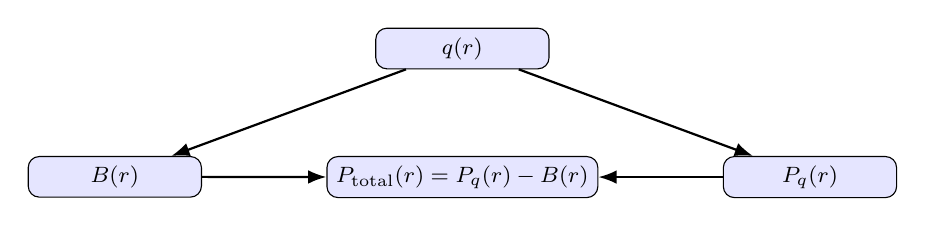
\begin{tikzpicture}[
    node distance=1.1cm and 2.2cm,
    every node/.style={align=center},
    box/.style={rectangle, draw, rounded corners, minimum width=2.2cm, minimum height=0.4cm, fill=blue!10, font=\footnotesize},
    arrow/.style={-{Latex}, thick}
  ]
  
  % Nodes
  \node[box] (qr) {\( q(r) \)};
  \node[box, below left=of qr] (Br) {\( B(r) \)};
  \node[box, below right=of qr] (Pq) {\( P_q(r) \)};
  \node[box, below=of qr] (Ptotal) {\( P_{\text{total}}(r) = P_q(r) - B(r) \)};
  
  % Arrows
  \draw[arrow] (qr) -- (Br);
  \draw[arrow] (qr) -- (Pq);
  \draw[arrow] (Br) -- (Ptotal);
  \draw[arrow] (Pq) -- (Ptotal);
\end{tikzpicture}
  \vspace{0.5cm}
{\footnotesize \color{black} \( q(r) \) determina tanto el confinamiento como la presión estadística, dando lugar a la presión total observada.}
\note{
\Large
\begin{itemize}
  \item En este diagrama resumo visualmente las relaciones clave entre las variables del modelo.
  \item El parámetro \( q(r) \) es la entrada principal: afecta tanto al término estadístico \( P_q(r) \) como al término de confinamiento \( B(r) \).
  \item Ambas cantidades se combinan para dar lugar a la presión total \( P_{\text{total}}(r) \), que es lo que finalmente se mide o se espera preservar.
  \item Este enfoque muestra cómo \( q(r) \) unifica dos aspectos del sistema: la termodinámica no extensiva y la física del confinamiento.
  \item Refuerza la idea de que el parámetro \( q \) no es simplemente libre, sino que lleva contenido físico del sistema.
\end{itemize}
}
\end{frame}

%%%%%%%%%%%%%%%%%%%%%%%%%%%%%%%%%%%%%%%%%%%%%%%%%%%%%%%%%%%%%%%%%%%%%%%%%%%%%%%%%%%%%
\section[Resultados]{6. Resultados}
\begin{frame}{Comparación con resultados de Lattice QCD}
  \begin{columns}
    % Columna izquierda: imagen
    \column{0.5\textwidth}
    \centering
    \includegraphics[width=\linewidth]{figures/LQCD_vs_TsallisMIT.png}
    \vspace{0.3em}
    \scriptsize \color{black} Comparación entre LQCD (Shanahan y Detmold) y el modelo Tsallis-MIT.

    % Columna derecha: texto
    \column{0.5\textwidth}
    \begin{itemize}
      \item Se comparan las distribuciones \( r^2 P(r) \) para distintas \( \mu \) en el modelo Tsallis-MIT.
      \item Buen acuerdo cualitativo con los resultados de Lattice QCD, en particular para \( r \lesssim 1.2 \, \text{fm} \).
      \item El modelo reproduce el pico en \( P(r) \) alrededor de \( r \sim 0.5 \, \text{fm} \), ajustando el parámetro \( q \).
    \end{itemize}
  \end{columns}
  \note{
\Large
\begin{itemize}
  \item Aquí muestro la comparación directa entre los resultados del modelo Tsallis-MIT y los obtenidos por Lattice QCD (trabajo de Shanahan y Detmold).
  \item El gráfico presenta la función \( r^2 P(r) \), que permite visualizar el perfil de presión en función del radio.
  \item Se observa que el modelo reproduce correctamente el pico de presión en \( r \sim 0.5 \, \text{fm} \), una característica clave del confinamiento.
  \item El ajuste del parámetro \( q \) permite modelar la forma de la curva con buena precisión hasta \( r \approx 1.2 \, \text{fm} \).
  \item Esto respalda el uso de estadística de Tsallis como una herramienta efectiva para describir confinamiento en QCD.
\end{itemize}
}
\end{frame}

\begin{frame}{Influencia del potencial químico}
  \begin{columns}
    % Columna izquierda: figura
    \column{0.5\textwidth}
    \centering
    \includegraphics[width=\linewidth]{figures/Pressure_mu_variation.png}
    \vspace{0.3em}
    \scriptsize \color{black} Distribución \( P_q(r) \) para distintos \( \mu \)

    % Columna derecha: texto
    \column{0.5\textwidth}
    \begin{itemize}
      \item Al incrementar \( \mu \), la presión repulsiva en el centro del protón aumenta.
      \item También se intensifica la presión negativa en la periferia.
      \item Esto sugiere un confinamiento más fuerte con mayor densidad bariónica.
      \item El modelo Tsallis-MIT captura correctamente estas variaciones internas.
    \end{itemize}
  \end{columns}
  \note{
\Large
\begin{itemize}
  \item En esta diapositiva analizo cómo cambia el perfil de presión \( P_q(r) \) al variar el potencial químico \( \mu \).
  \item Vemos que al aumentar \( \mu \), crece la presión repulsiva cerca del centro, lo que es consistente con una mayor presencia de quarks.
  \item Simultáneamente, la región de presión negativa también se vuelve más profunda, lo que indica un confinamiento más intenso.
  \item Este comportamiento es un buen indicador de que el modelo responde adecuadamente a cambios en la densidad bariónica del sistema.
  \item Resalto que el parámetro \( q \) y el perfil \( B(r) \) permiten describir estas variaciones de forma dinámica.
\end{itemize}
}
\end{frame}

\begin{frame}{Reconstrucción de la presión de gluones}
  \begin{columns}
    % Columna izquierda: figura
    \column{0.5\textwidth}
    \centering
    \includegraphics[width=\linewidth]{figures/Pressure_gluons_reconstructed.png}
    \vspace{0.3em}
    \scriptsize \color{black} Reconstrucción de la presión de gluones

    % Columna derecha: contenido explicativo
    \column{0.5\textwidth}
    \begin{itemize}
      \item Usamos la relación:
      \[
        P_{\text{gluones}}(r) = P_{\text{total}}(r) - P_{\text{quarks}}(r)
      \]
      \item Interpretamos \( P_{\text{gluones}}(r) \) como el mar de fondo gluónico.
      \item Este mar es responsable de la presión de bolsa efectiva.
      \item El perfil muestra:
      \begin{itemize}
        \item Disminución con el radio \( r \).
        \item Mayor contribución en la periferia del protón.
      \end{itemize}
    \end{itemize}
  \end{columns}
  \note{
\Large
\begin{itemize}
  \item En esta diapositiva mostramos cómo se puede reconstruir la presión de gluones restando la presión de quarks a la presión total.
  \item Esto nos da una idea del mar gluónico que rodea a los quarks y que actúa como entorno de confinamiento.
  \item El perfil reconstruido de \( P_{\text{gluones}}(r) \) presenta un comportamiento decreciente con el radio, lo cual es consistente con un entorno externo que actúa hacia el interior.
  \item Se observa que esta presión gluónica tiene mayor peso en las regiones periféricas del protón, reforzando la idea de un cascarón que contribuye al confinamiento.
  \item Esta reconstrucción permite interpretar \( B(r) \) no solo como una constante fenomenológica, sino como una manifestación del entorno gluónico dinámico.
\end{itemize}
}
\end{frame}

%%%%%%%%%%%%%%%%%%%%%%%%%%%%%%%%%%%%%%%%%%%%%%%%%%%%%%%%%%%%%%%%%%%%%%%%%%%%%%%%%%%%%
\section[Exploraciones adicionales]{7. Exploraciones adicionales}

\begin{frame}{Perspectiva futura: masas hadrónicas con estadística de Tsallis}
  \begin{itemize}
    \item El modelo de bolsa tradicional (MIT) permite calcular masas hadrónicas mediante:
    \[
      M = \sum_i \omega_i + \frac{4}{3} \pi R^3 B + \Delta E_{\text{int}} - \frac{Z_0}{R}
    \]
    \item Modelos más recientes (Joseph \& Nair, 1981) proponen que \( B \) depende de la densidad.
    \item Nuestra propuesta: sustituir las contribuciones energéticas por expresiones derivadas de la estadística de Tsallis.
    \item Preguntas clave:
    \begin{itemize}
      \item ¿Qué valor de \( q \) reproduce la masa del protón?
      \item \item ¿Qué perfil \( q(r) \) conduce a un mínimo energético compatible con la masa del protón?
    \end{itemize}
  \end{itemize}
  \note{
\Large
\begin{itemize}
  \item En esta última diapositiva presento la dirección que podría tomar este trabajo en el futuro.
  \item El modelo de bolsa tradicional permite estimar masas hadrónicas sumando energía de modos, energía de volumen, interacción y correcciones finitas.
  \item Sin embargo, hay propuestas como la de Joseph y Nair donde la presión de bolsa \( B \) se modela como dependiente de la densidad, lo que introduce mayor realismo.
  \item Nuestra idea es ir más allá: sustituir la energía de los modos y la presión de bolsa por expresiones derivadas directamente de la estadística de Tsallis.
  \item Esto permitiría obtener una masa como función explícita del parámetro \( q \), es decir, vincular la masa observada con condiciones no extensivas del sistema.
  \item Las preguntas centrales que surgen son: ¿Qué valor de \( q \) da como resultado la masa del protón? ¿Y qué perfil espacial \( q(r) \) minimizaría la energía total?
  \item Esto abre una vía para estudiar no solo las propiedades termodinámicas del protón, sino también su estructura de masa desde una perspectiva más fundamental.
\end{itemize}
}
\end{frame}


\begin{frame}{Modelo alternativo basado en \( F_q \)}
  \begin{itemize}
    \item Enfoque desarrollado por mi asesor junto con otro de sus estudiantes.
    \item A partir de la entropía \( S_q \), se calcula la energía libre de Helmholtz:
    \[
    F_q = -k_{\mathrm{B}} T \ln_q \Xi
    \]
    \item La energía interna se recupera con:
    \[
    U_q = F_q + T S_q
    \]
    \item Ajustan \( q \) para que \( U_q \approx M_{\text{exp}} \).
    \item No exploran perfiles espaciales de \( q(r) \) ni presión.
  \end{itemize}

  \note{
  \Large
  \begin{itemize}
    \item Este enfoque fue desarrollado por mi asesor junto con otro de sus estudiantes, como parte de un trabajo previo.
    \item Parte de la entropía no extensiva \( S_q \), desde donde calculan la energía libre de Helmholtz \( F_q \) usando el logaritmo \( q \)-generalizado.
    \item Posteriormente recuperan la energía interna \( U_q \), que depende tanto de \( F_q \) como de \( S_q \).
    \item Ajustan el valor del parámetro \( q \) para que la energía interna coincida con la masa experimental del protón.
    \item Sin embargo, este enfoque no considera perfiles espaciales \( q(r) \) ni evalúa distribuciones de presión.
    \item Mi propuesta amplía esta perspectiva al vincular \( q \) con propiedades dinámicas del confinamiento.
  \end{itemize}
  }
\end{frame}


\begin{frame}{Línea de desarrollo futuro: masas con estadística de Tsallis}
  \centering
  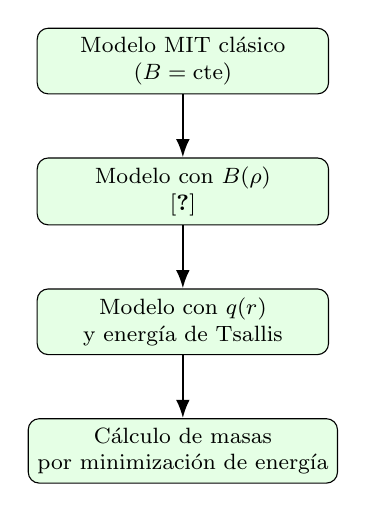
\begin{tikzpicture}[
    node distance=0.8cm and 2.2cm, % Reducido de 1.1cm a 0.8cm
    every node/.style={align=center},
    box/.style={rectangle, draw, rounded corners, minimum width=3.7cm, minimum height=0.6cm, fill=green!10, font=\footnotesize}, % altura y fuente más pequeñas
    arrow/.style={-{Latex}, thick}
  ]

  \node[box] (MIT) {Modelo MIT clásico \\ (\( B = \text{cte} \))};
  \node[box, below=of MIT] (JNAIR) {Modelo con \( B(\rho) \) \\ \cite{Joseph1981}};
  \node[box, below=of JNAIR] (TSALLIS) {Modelo con \( q(r) \) \\ y energía de Tsallis};
  \node[box, below=of TSALLIS] (MASSES) {Cálculo de masas \\ por minimización de energía};

  \draw[arrow] (MIT) -- (JNAIR);
  \draw[arrow] (JNAIR) -- (TSALLIS);
  \draw[arrow] (TSALLIS) -- (MASSES);

\end{tikzpicture}
\note{
\Large
\begin{itemize}
  \item Este diagrama resume la evolución de modelos hacia una descripción más realista del confinamiento.
  \item El modelo original del MIT asume una presión de bolsa constante, \( B = \text{cte} \), sin depender de la densidad ni el entorno.
  \item Joseph y Nair propusieron que \( B \) puede depender de la densidad bariónica \( \rho \), añadiendo un componente dinámico.
  \item Nuestro enfoque incorpora la estadística de Tsallis y propone que \( q \) varía espacialmente como \( q(r) \), lo cual permite capturar efectos de correlación y confinamiento.
  \item Finalmente, esta estructura permite usar un criterio de energía mínima para calcular masas hadrónicas a partir del perfil de \( q(r) \).
\end{itemize}
}
\end{frame}

\begin{frame}{Exploración adicional: energía y confinamiento}
  \begin{itemize}
    \item Se propuso relacionar la masa del hadrón con la energía interna obtenida desde Tsallis:
    \[
      U_q = \frac{37 \pi^2}{30} V T^4 + \frac{128 \pi^4}{225} (1 - q) V^2 T^7
    \]
    \item Derivada a partir de:
    \begin{itemize}
      \item \( F_q \): energía libre de Helmholtz
      \item \( S_q \): entropía no extensiva del sistema quark-gluón
    \end{itemize}
    \item Se intentó igualar \( U_q \approx M_{\text{bag}} \) para despejar \( q \).
    \item Resultado: despeje trivial, pues \( V \) y \( T \) ya están fijados por la geometría.
  \end{itemize}
  \note{
\Large
\begin{itemize}
  \item En esta sección presento una exploración alternativa para conectar energía interna y masa del hadrón.
  \item La idea fue usar la energía interna \( U_q \) obtenida desde la estadística de Tsallis y proponer que esta debe coincidir con la masa efectiva del protón.
  \item La expresión incluye un término extensivo en \( T^4 \) y una corrección no extensiva proporcional a \( (1 - q) V^2 T^7 \).
  \item Se parte de la energía libre \( F_q \) y la entropía \( S_q \), aplicando la relación \( U_q = F_q + T S_q \).
  \item Aunque la propuesta es válida formalmente, el resultado es poco útil en la práctica porque el volumen \( V \) y la temperatura \( T \) ya están determinados por la cavidad esférica.
  \item Por tanto, el parámetro \( q \) no queda restringido, lo que motiva explorar otras rutas donde \( q \) tenga una dependencia funcional o espacial.
\end{itemize}
}
\end{frame}

\begin{frame}{Conclusión de esta exploración}
  \begin{itemize}
    \item Intención: reinterpretar la energía de confinamiento como una propiedad emergente del formalismo de Tsallis.
    \item Dificultades:
    \begin{itemize}
      \item Los parámetros \( V \) y \( T \) no permiten libertad para determinar \( q \).
    \end{itemize}
    \item Futuro:
    \begin{itemize}
      \item Incorporar la estadística de Tsallis en la cuantización de modos.
      \item Reformular las contribuciones energéticas del modelo de bolsa desde una base no extensiva.
    \end{itemize}
  \end{itemize}
  \note{
\Large
\begin{itemize}
  \item Concluyo esta exploración destacando que el objetivo era reinterpretar la energía de confinamiento como un efecto emergente de la estadística no extensiva.
  \item Aunque la idea es interesante, nos enfrentamos a una limitación importante: los parámetros \( V \) y \( T \) ya están fijados por la geometría del sistema, lo que deja a \( q \) sin capacidad para ajustarse libremente.
  \item Esto sugiere que no es suficiente con igualar la energía interna a la masa; se necesita una reformulación más profunda.
  \item En el futuro, propongo abordar el problema desde la cuantización de los modos dentro del formalismo de Tsallis.
  \item También será necesario replantear el modelo de bolsa desde su base, para que las contribuciones energéticas reflejen directamente la no extensividad.
\end{itemize}
}
\end{frame}

%%%%%%%%%%%%%%%%%%%%%%%%%%%%%%%%%%%%%%%%%%%%%%%%%%%%%%%%%%%%%%%%%%%%%%%%%%%%%%%%%%%%%
\section[Conclusiones]{8. Conclusiones}
\begin{frame}{Conclusión general del trabajo}
  \begin{itemize}
    \item Se propuso una interpretación estadística del confinamiento hadrónico mediante el parámetro \( q \) de Tsallis.
    \item Se desarrolló un modelo mixto: estadística no extensiva + geometría esférica de bolsa con presión espacialmente dependiente.
    \item Se introdujo la función \( q(r) \) como descriptor dinámico del confinamiento, en lugar de asumir una constante de bolsa \( B \).
  \end{itemize}
\end{frame}

\begin{frame}{Resultados principales}
  \begin{itemize}
    \item Se obtuvieron perfiles de presión \( P_q(r) \) para quarks y gluones con estadística de Tsallis.
    \item Se reconstruyó \( B(r) \) desde configuraciones térmicas en cavidades esféricas.
    \item Se simuló \( B(q, r) \) y se identificó una relación funcional invertible entre \( B \) y \( q \).
    \item Se justificó físicamente la posibilidad de interpretar \( q(r) \) como medida del confinamiento.
  \end{itemize}
\end{frame}

\begin{frame}{Implicaciones físicas del modelo}
  \begin{itemize}
    \item El parámetro \( q \) deja de ser solo un índice de no extensividad abstracto y adquiere significado físico concreto.
    \item El confinamiento se describe como efecto estadístico emergente, y no como un potencial externo arbitrario.
    \item El modelo propuesto respeta la termodinámica, la simetría esférica y las condiciones límite del protón.
  \end{itemize}
\end{frame}

\begin{frame}{Líneas futuras de investigación}
  \begin{itemize}
    \item Generalizar el modelo a sistemas tridimensionales sin simetría esférica.
    \item Explorar la cuantización de modos en cavidades con estadística de Tsallis.
    \item Calcular las masas hadrónicas a partir de energías obtenidas con el modelo \( q(r) \).
    \item Extender la formulación a condiciones de temperatura y densidad extremas (plasma QGP).
  \end{itemize}
\end{frame}

% \begin{frame}{Mensaje final}
%   \centering
%   \Large
%   El confinamiento ya no se describe sólo por una constante, \\[0.3cm]
%   sino por una función estadística que evoluciona radialmente: \\[0.5cm]
%   \textbf{\huge\( \boxed{q(r)} \)} \\[0.5cm]
%   \normalsize
%   Una nueva puerta hacia una estadística del interior hadrónico.
% \end{frame}

\begin{frame}[standout]
  \centering
  \Large ¡Gracias por su atención!
  \centering
  \Huge ¿Preguntas?
\end{frame}

% Bibliografía si aplica
\appendix
\begin{frame}[allowframebreaks]{Bibliografía}
  \printbibliography
\end{frame}
% Run with
% pdfpc presentation.pdf --notes=right
\end{document}